\chapter{Implementation}
\label{chap:implementation}
In this chapter, we will introduce the implementation of our method. We will focus on a GPU-oriented implementation of the method presented in Chapter \ref{chap:method}. First, we will briefly introduce the environment in which we are operating. Then, we will give a general outline of our algorithm. Then, we will discuss in more detail some of the ideas introduced in the outline. After this discussion, we will discuss some defects and artifacts in our algorithm that arose during the implementation, and how we have solved them. Finally, we will extend our implementation to different kind of lights. Finally, we will discuss our implementation.

\section{Environment}

In order to justify some of the choices and the code parts that will be introduced in this section, we will first introduce the environment of our implementation. The method we are going to discuss was made using the OpenGL API, version 4.3 (released in August 2012), a multi-platform API used for rendering 2D and 3D accelerated graphics. With the OpenGL API comes GLSL, the \emph{OpenGL Shading Language}, used for writing pieces of code to be run on the GPU, called \emph{shaders}. Our method uses some advanced features of OpenGL 4.3, so it is not immediately portable to previous generation hardware, and runs only on high-end modern GPUs. On the CPU side, we use an extended framework based on Qt, a C++ library that allows to create a OpenGL context and graphical interfaces in an easy way.

\section{Algorithm overview}

By keeping the limitations presented in Chapter \ref{chap:intro} in mind, we introduce our algorithm. The algorithm is inspired by \emph{translucent shadow maps} \citep{Dachsbacher:2003:TSM:882404.882433}, that we presented in Chapter \ref{chap:previous}. The general idea is to first render the scene from the light point of view, then place the disk we discussed in the previous Chapter (Section \ref{sec:m_overv}) directly on the generated texture, storing the result in a radiance map. We use many directions in order to capture all the sides of the object. Finally, we sample from the obtained radiance map for the final rendering.

In this section, we will assume to only have one directional light with radiance $L_d$ and direction $\vomega_d$, with one not-deformable object in the scene. We will discuss later how to extend the method to multiple light sources.

\textbf{Step 1 - Light buffer} \\
In the first step, positions and normals of the object are rendered into a texture from the light point of view. We will refer to the resulting texture as the \emph{light map}. As in standard shadow mapping we create and store a matrix to convert between world space and texture light space. Depth testing in this step is enabled. More details on the implementation of a render to texture are presented in Section \ref{sec:rendertotexture}.

\begin{figure}[!ht]
\centering
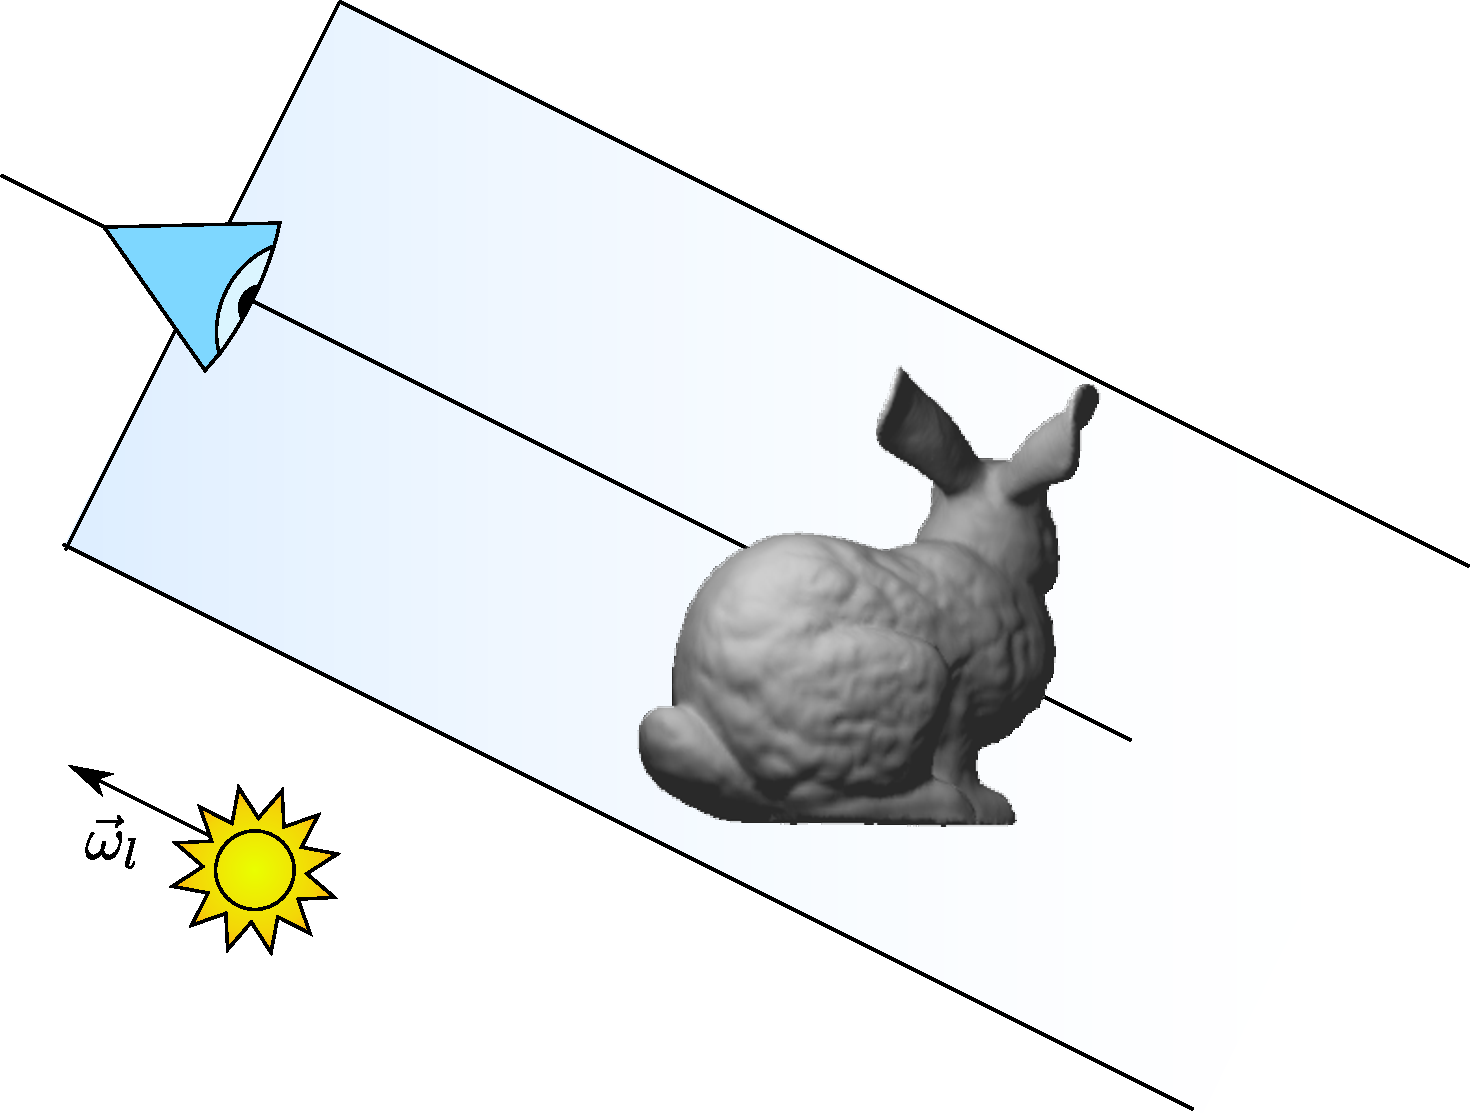
\includegraphics[width=0.8 \linewidth]{images/method/step1.pdf}
\caption{Render to G-buffer. Note that the frustum and the light direction are aligned.}
\label{fig:step1}
\end{figure} 

\begin{figure}
\centering
\subfloat[{Vertex buffer}]{
  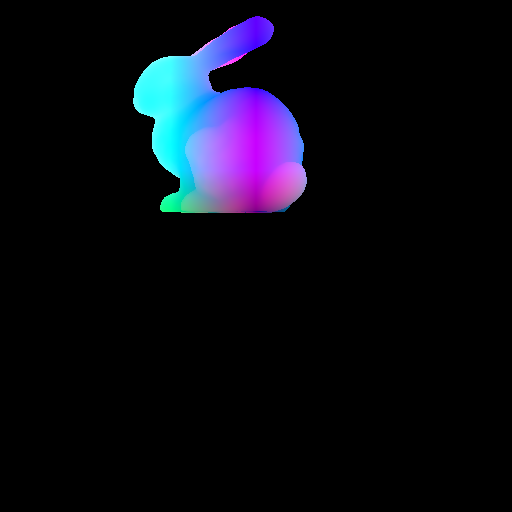
\includegraphics[width=0.5 \linewidth]{images/method/vertices.png}
  \label{fig:vbuff}
}
\subfloat[{Normal buffer}]{
  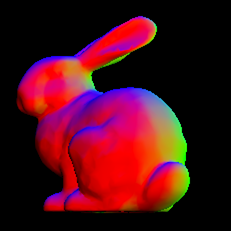
\includegraphics[width=0.5 \linewidth]{images/method/normals.png}
  \label{fig:nbuff}
} 
\label{fig:lightbuffers}
\caption{State of the vertex and normal buffer after rendering from a directional light. The model used was the Stanford bunny from the Standford 3D Scanning repository.}
\end{figure}
\FloatBarrier
\textbf{Step 2 - Render to radiance map} \\
In the second step, we render the object from $K$ different directions into another texture, called the \emph{radiance map}. The radiance map is organized as a layered texture, where each layer represents a direction. More details on render to texture and layered textures are presented in sections \ref{sec:rendertotexture} and \ref{sec:layeredrendering}. The points on which to place the cameras are chosen randomly, distributed on a sphere (see Section \ref{sec:random} for the details). The cameras point towards the center of the object bounding box.

On this step, for each pixel that corresponds to an exiting point $\x_o$ the shader samples $N$ points from the texture rendered in the previous step. If the sampled point is valid, it is then used to calculate the BSSRDF and accumulate it in the resulting radiance map. So, this step calculates the following:
$$
R^{k}(\x_o) = L_d \sum_{i = 1}^N S(\x^{k}_i, \vomega_l, \x_o, \vomega_o) \exp\left(\sigma_{tr} r^{k}_i\right), \ \ k \in [0,K-1] 
\label{eq:evolution_step}
$$

\begin{figure}[!ht]
\centering
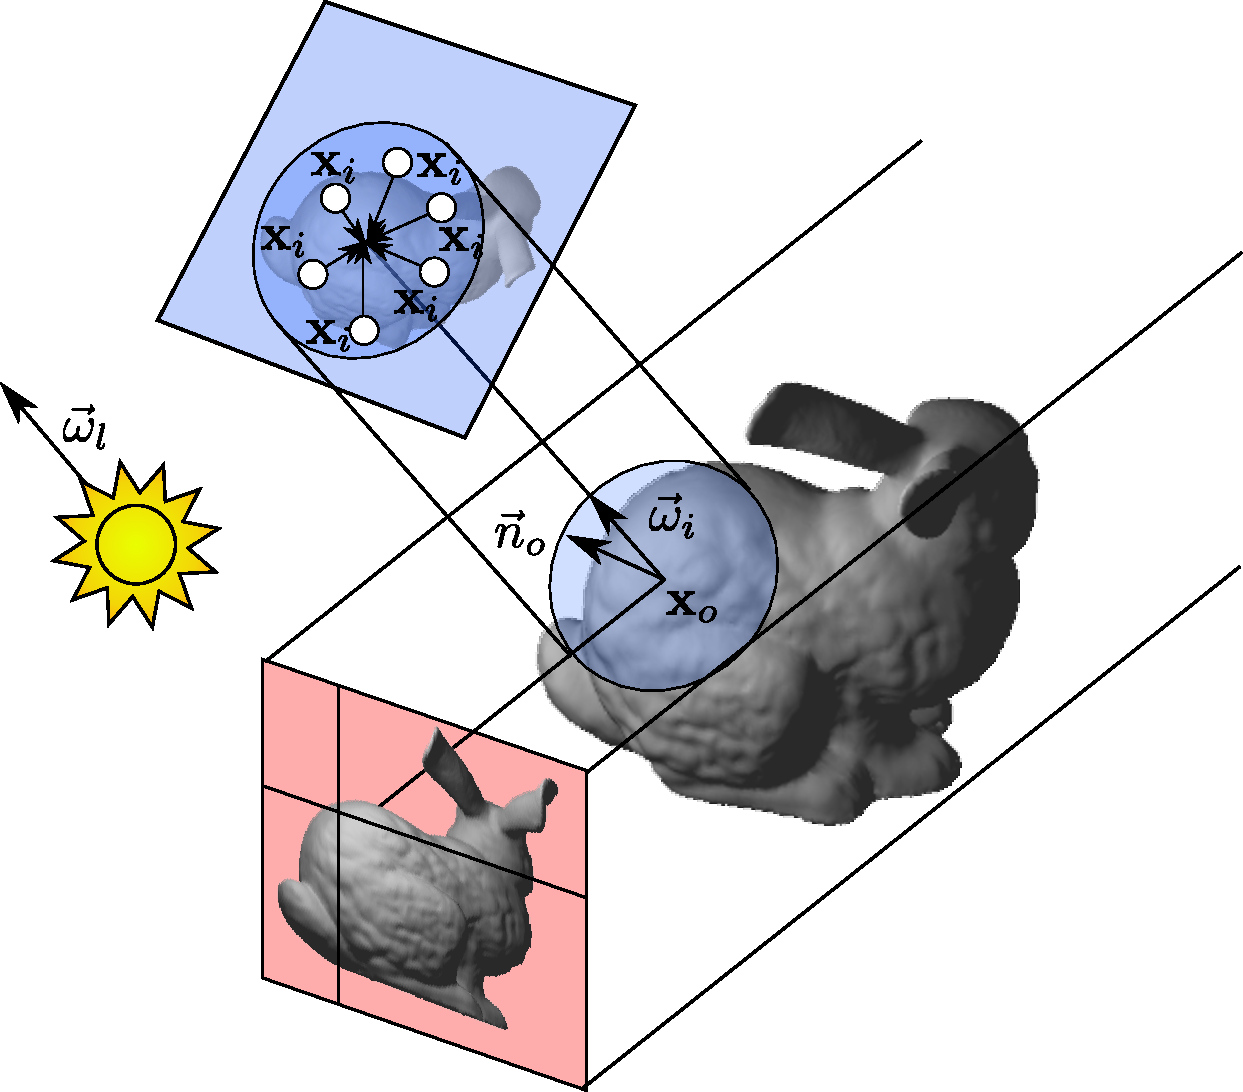
\includegraphics[width=0.9 \linewidth]{images/method/step2_improved.pdf}
\caption{Render to the radiance map. When we render the point $\x_o$, the position in the light map is calculated and the values $\x_i$ in the samples are calculated and summed over.}
\label{fig:step2}
\end{figure} 

Where we recall that we have introduced an exponential term in order to compensate for the exponential displacement of the sampling pattern. The generation of the sampling pattern is described in Section \ref{sec:exponentiallybiased} in more detail. We introduced a $k$ parameter, that represents the current direction we are rendering to. We can see how we are rendering a point from one of the considered directions in Figure \ref{fig:stepfrustum}. Also in this case, the texture space - world space conversion matrices are stored and prepared to be reused in step 3, where we will combine the results. 

We can appreciate that rendering the light from the camera point of view comes with two important advantages:
\begin{itemize}
\item If the disk is placed in texture space, it is automatically oriented towards the light direction, that is $\vomega_d = \vomega_l$.
\item The light renders in the texture only the points directly visible from it, that are also the only points directly lit. In addition, if we sample the light map on any point, we get the corresponding vertex that is closest to the light.
\end{itemize}
This two factors allows us to sample the most optimal point and direction in where to place the disk, as we described it in Section \ref{sec:m_overv}.
 
\begin{figure}[!ht]
\centering
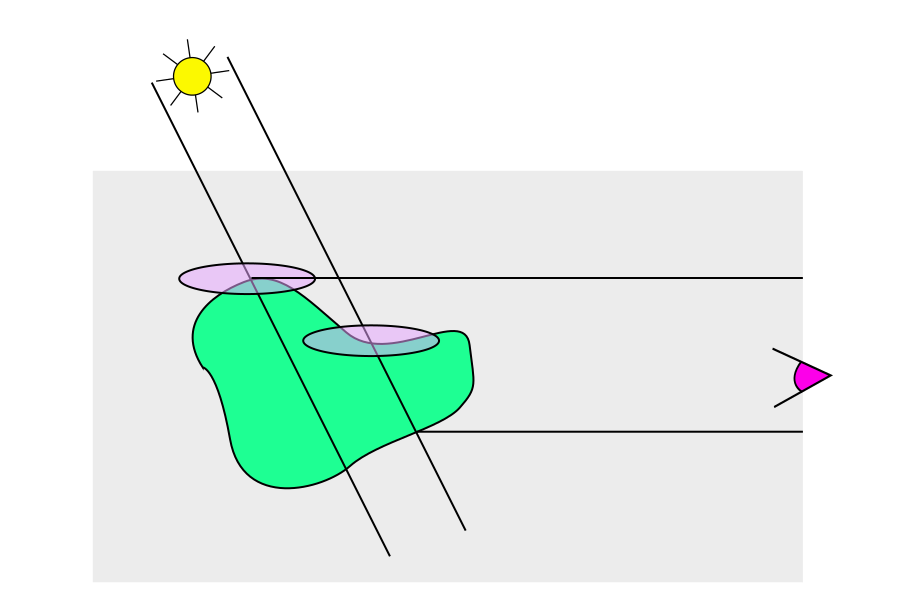
\includegraphics[width=\linewidth]{images/method/step2}
\caption{Render to cubemap, side view. The gray area represents the frustum of the current direction's camera (orthographic). We have three different cases of a point on the surface: $\x_o^1$ is visible from both the light and the camera, so the disk is placed on it. $\x_o^2$ is visible from the camera but not from the light, so the disk is placed in the closest position to the light. $\x_o^3$ is not visible from the camera, so it is discarded.}
\label{fig:stepfrustum}
\end{figure} 

In addition, on each layer, we accumulate the result over different frames:
$$
\tilde{R}^{t,k} = \sum_{i = 0}^{t-1} R^{i,k} + R^{t,k} = \tilde{R}^{t-1, k} + R^{t,k}
$$
$\tilde{R}$ here represents the value that is stored in the radiance map. In equation \ref{eq:evolution_step}, we omitted the dependence from time for the sake of clarity. We need an accumulation process in order to deal with the fact that the result from the previous computation are not reaching a satisfying result within one frame, so they need to be accumulated over a period of $T$ frames in order to reach an appreciable result. In order to do this, the sampled points need to change on different frames (in Section \ref{sec:random} we give more details on the process). 

Naturally, the accumulation process works only if the scene does not change. A change can be a relative change of positions between the points on the model and the light, so if the model gets translated, rotated or scaled, the accumulated result has to be discarded and the accumulation started all over. The directional cameras are locked with the model, so the pixels are always aligned. This is why in equation \ref{eq:evolution_step} the dependence from time of the point $\x_o$ and $\vomega_o$ have been dropped. 
 
\textbf{Step 3 - Combination} \\
In this step, we render of our model. Using the matrices and the textures prepared in the previous step, for each fragment on the surface we sample all the layers in the texture as illustrated in Figure \ref{fig:step3}. In order to do this, we need also to sample the depth map generated in the previous step. We can define this sampling as a visibility function to test if a point $\x$ belongs to layer $k$:
$$
V^k(\x) = \begin{cases}
1 & \text{if $\x$ is visible from the $k$th camera} \\
0 & \text{otherwise}
\end{cases}
$$
The function $V$ is calculated by sampling the k-th layer depth map in a way similar to shadow mapping (details in Section \ref{sec:shadow_map}). Given this function, we can simply represent the outgoing radiance by simply averaging the summation over the $K$ layers:
$$
L_{SS}^t(\mathbf{x}) = \frac{A_c}{N (t)} \frac{\displaystyle\sum_{k = 0}^{K-1}V^k(\x) \tilde{R}^{t,k}(\mathbf{x})}{\displaystyle\sum_{k = 0}^{K-1}V^k(\x)}
$$
The first factor $\frac{1}{t}$ is to average over the number of frames, while the second is the average area of a sample in the circle $\frac{A_c}{N}$, that is necessary to complete equation \ref{eq:inter2}. We note that we moved all the layer-independent computation into the final computation step, in order to save as much performance as possible. 

\begin{figure}[!ht]
\centering
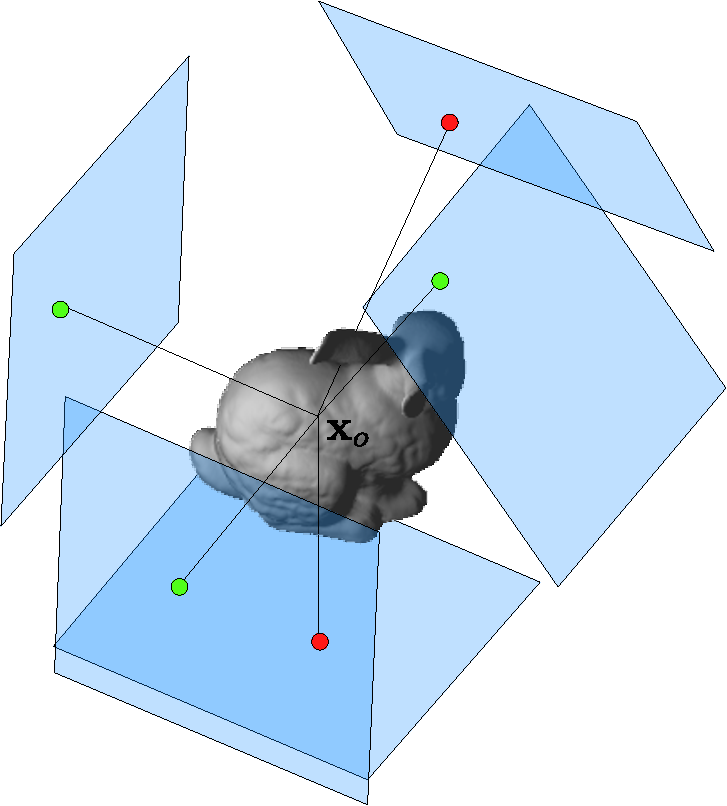
\includegraphics[width=0.6 \linewidth]{images/method/combination.pdf}
\caption{Final combination step. The blue quads indicates each one of the radiance map layers, as seen from their direction. We can see that in the point $\x_o$ the contribution from three faces (green dots) is considered. For the remaining two faces (red dots), the contribution is not considered as the point is not visible.}
\label{fig:step3}
\end{figure} 

We are not done yet, as for now we have computed the radiance only deriving from subsurface scattering. For finally describing the illumination of our scene, we need also to include a factor based on the surface reflection. Since the subsurface scattering radiance is already multiplied by a transmittance Fresnel term (in the BSSRDF equation in \ref{eq:bssrdfgen}) $T(\eta,\vomega_o)$ we the reflection color multiplied by the converse transmission term $1 - T(\eta,\vomega_o)$:
$$
L^t(\x, \vomega_o) = L_{SS}^t(\x) + (1 - T(\eta,\vomega_o)) L_i(\x, \vomega_o - 2 (\vomega_o \cdot \vec{n}) \vec{n})
$$
$L_i$ can be the radiance coming from other objects or by an environment map. After this, we just need to perform gamma correction in order to get the final result. Given the gamma coefficient $\gamma$, we perform gamma correction by:
$$
L_{gamma}^t(\x, \vomega_o, \gamma) = L^t(\x,\vomega_o)^{\frac{1}{\gamma}}
$$
And, adter this, we can finally send the radiance to the output device.
\begin{figure}[!ht]
\centering
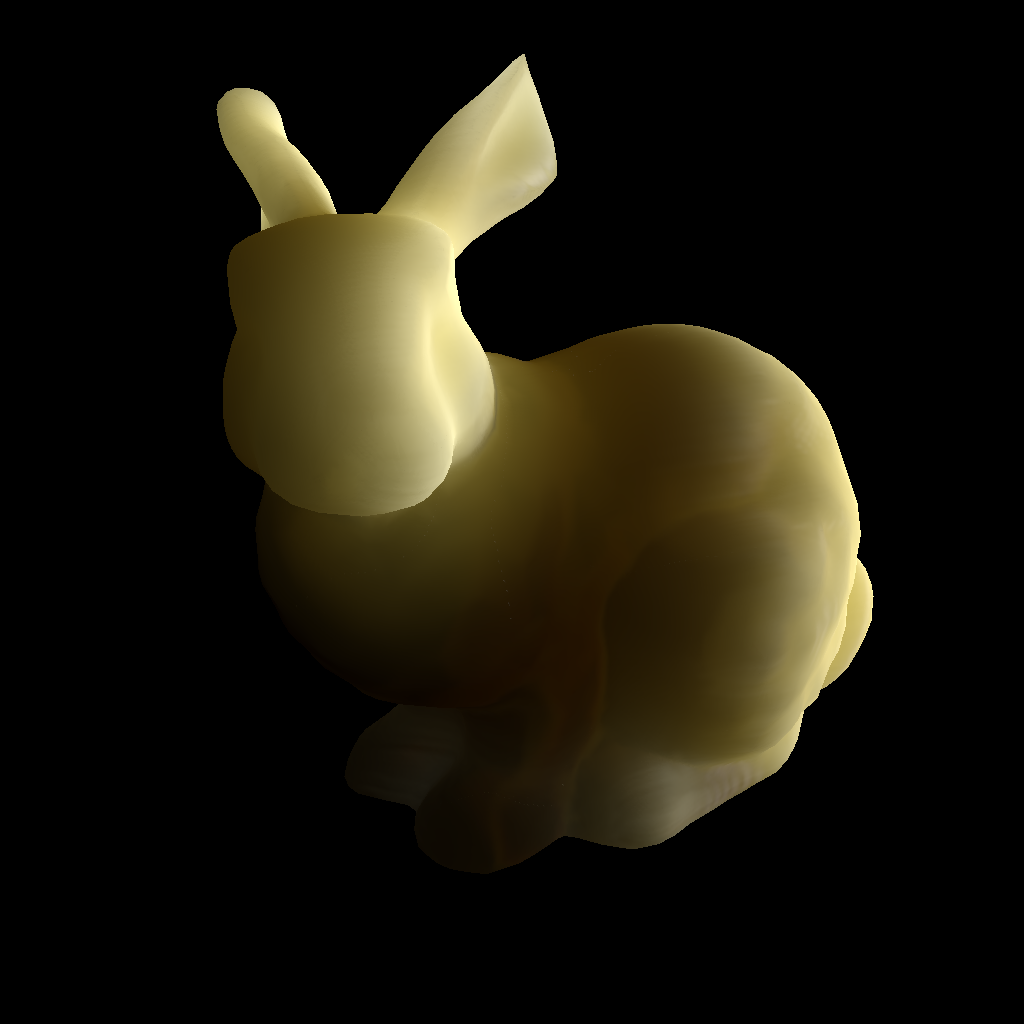
\includegraphics[width=0.8 \linewidth]{images/results/potato_100_convergence.png}
\caption{Final Result of the method after 100 frames simulating a potato bunny of dimensions $\approx 30 cm$. The parameters used were $r = 1 dm$, $N = 128$. All the results presented in this chapter are gamma corrected with $\gamma = 2.2$.}
\label{fig:potato_result}
\end{figure} 
\begin{figure}[!ht]
\centering
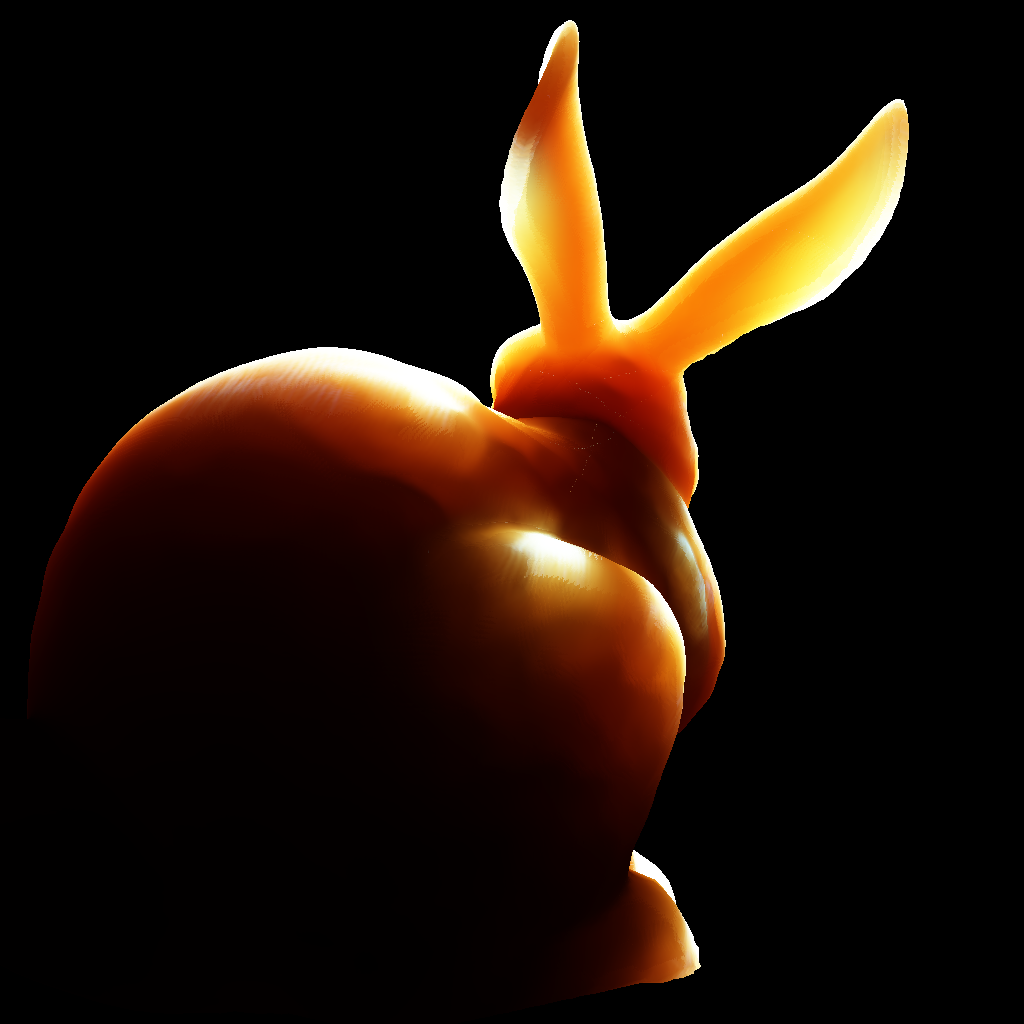
\includegraphics[width=0.8 \linewidth]{images/results/beer_backlit_100_convergence.png}
\caption{Final Result of the method after 100 frames simulating a backlit bunny made of beer, dimensions $\approx 30 cm$. The parameters used were $r = 3 dm$, $N = 128$.}
\label{fig:beer_result}
\end{figure} 

\section{Implementation details}
In this section, we will further expand the overview given in the previous section by adding further details. We organized this section in topics, in each one of them expanding a particular aspect of our algorithm. Each point clarifies with examples one technique or approach used in the method. The code given on each example does not necessarily come from our implementation, but it can be simplified for illustration purposes.

\subsection{Render-to-texture}
\label{sec:rendertotexture}
In a graphics API, and more specifically in OpenGL, all the output from a final shader stage is usually sent to the display device in order to be displayed on the screen. However, it is possible to redirect the output into another memory area of the GPU and reuse it for further computations. This allows to create complicated rendering techniques such as the one described in this report. 

In OpenGL, is possible to redirect the output to a texture object. We can do this through a so-called \emph{framebuffer object} (FBO). A FBO is a collection of objects that allows off-screen rendering. A FBO has \emph{attachment points}, to which we can attach textures. A texture can be attached to one of the output color channels of the fragment shader (\gl{GL_COLOR_ATTACHMENT0}, \gl{GL_COLOR_ATTACHMENT1}, ...), to the depth buffer output (\gl{GL_DEPTH_ATTACHMENT}) or to the stencil buffer output (\gl{GL_STENCIL_ATTACHMENT}).

The connection between the framebuffer and the texture can be set in a initialization step (listing \ref{lst:rendertotextureinit}). Then, by simply binding the FBO (listing \ref{lst:rendertotexturerender}) we redirect our screen output to the desired texture.

\begin{lstlisting}[language=C++,label=lst:rendertotextureinit,caption={Render to texture example, initilalization phase. Note the call to \gl{glFramebufferTexture2D}}]
GLuint tex,fbo;
// Generating texture
glGenTextures(1, &tex);
glBindTexture(GL_TEXTURE_2D, tex);
[...] // setting up texture parameters...
glTexImage2D(GL_TEXTURE_2D, 0, GL_RGBA16F, size, size, 0, GL_RGBA, GL_FLOAT, 0);

glGenFramebuffers(1,&fbo);

// connecting current fbo and texture
glBindFramebuffer(GL_DRAW_FRAMEBUFFER, fbo);
glFramebufferTexture2D(GL_DRAW_FRAMEBUFFER, GL_COLOR_ATTACHMENT0, GL_TEXTURE_2D, tex, 0);
glBindFramebuffer(GL_DRAW_FRAMEBUFFER, 0); //Binding back main framebuffer
\end{lstlisting}

\begin{lstlisting}[language=C++,label=lst:rendertotexturerender,caption={Render to texture example, rendering phase. Since we have not configured and FBO for depth and stencil buffers, depth testing and stencil should be disabled at this point.}]
glBindFramebuffer(GL_DRAW_FRAMEBUFFER, fbo);
GLenum buffers[] = {GL_COLOR_ATTACHMENT0};
glDrawBuffers(1, buffers);
[...] // draw model
\end{lstlisting}

\subsection{Layered rendering}
\label{sec:layeredrendering}
Layered rendering is a special feature used to render to a special type of texture called \emph{layered texture}. Let us take as an example the step 2 of our algorithm, where we need to render the object from $K$ different directions. A first approach to this would be to create $K$ 2D textures of type \gl{GL_TEXTURE_2D}, and perform $K$ draw calls, rebinding the texture on the current FBO each time. OpenGL, however, provides a way to do this with a single draw call, potentially reducing the rendering costs due to context switching.

We will use the OpenGL provided type \gl{GL_TEXTURE_2D_ARRAY}, that we initialize in the usual way, noting that an array texture should be allocated as a 3D texture. When binding it to an FBO, we use the generic \gl{glBindFramebufferTexture}:
\begin{lstlisting}[language=C++,label=lst:initarraytexture,caption={Initializing array texture. Note that the number of layers is passed to the \gl{glTexStorage3D} command.}]
GLuint fbo, arraytex;
glGenFramebuffers(1,&fbo);
glGenTextures(1, &arraytex);

glBindTexture(GL_TEXTURE_2D_ARRAY, arraytex);
[...] // setting up texture parameters, omitted
glTexStorage3D(GL_TEXTURE_2D_ARRAY, levels, GL_RGBA32F, size, size,layers);

glBindFramebuffer(GL_DRAW_FRAMEBUFFER, fbo);
glFramebufferTexture(GL_DRAW_FRAMEBUFFER, GL_COLOR_ATTACHMENT0, arraytex, 0);
\end{lstlisting}
In order to render to a layered texture, we need then to introduce a geometry shader. In our example, the difference between each layer is basically a different view matrix. So, we move the computation of the position, usually left to the vertex shader, to the geometry shader. We first introduce the code:

\begin{lstlisting}[language=GLSL,label=lst:arraygeomshader,caption={Geometry shader for layered rendering. The multiplication by the model matrix of vertex v is performed in the vertex shader (not shown).}]
#version 430
#define DIRECTIONS 16
layout(triangles) in;
layout(triangle_strip, max_vertices = 60) out;

uniform mat4 P;
uniform mat4 viewMatrices[DIRECTIONS];

void main(void)
{
    for(int i = 0; i < DIRECTIONS; i++)
    {
        gl_Layer = i;

        for(int k = 0; k < 3; k++)
        {
            vec4 v = gl_in[k].gl_Position;
            gl_Position = P * viewMatrices[i] * v;
            EmitVertex();
        }
        EndPrimitive();
    }
}
\end{lstlisting}

\begin{figure}[!ht]
\centering
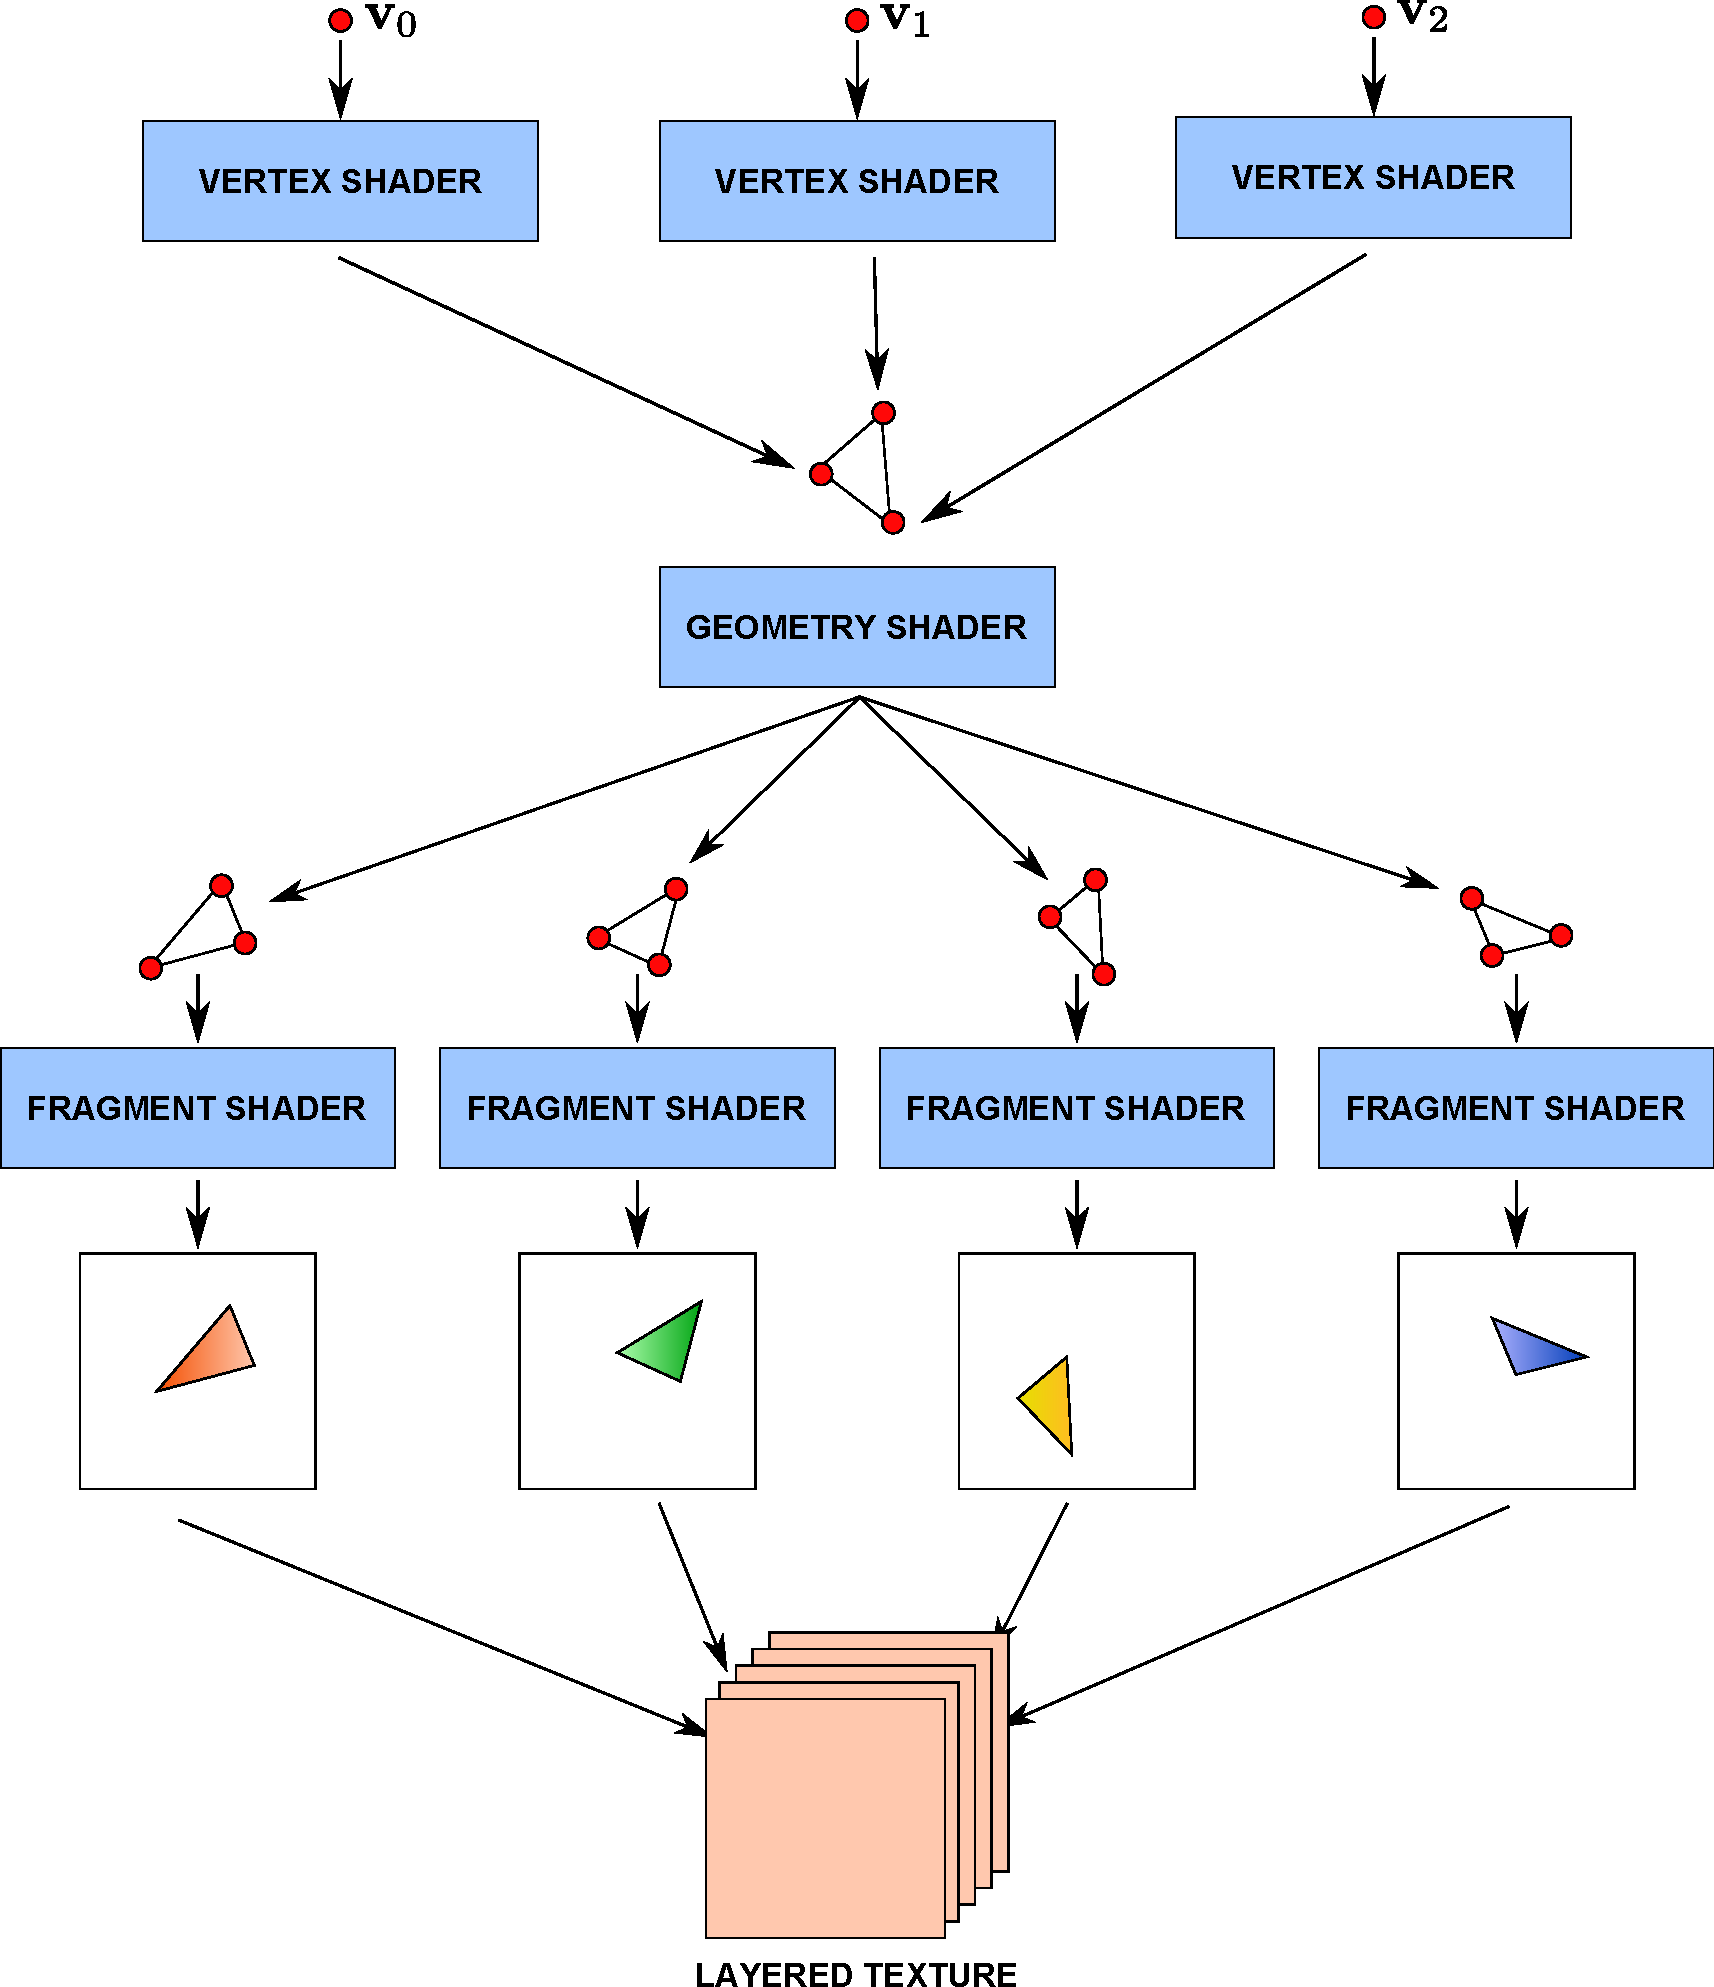
\includegraphics[width=\linewidth]{images/method/layered.pdf}
\caption{Diagram that illustrates layered rendering.}
\label{fig:layered}
\end{figure} 

As we can see, we duplicate each one of the incoming triangles and then output it multiplied by a different view matrix. the \gl{EndPrimitive()} function ensures that the output triangles in the final triangle strip are separated. In order to render each triangle to a different layer, we need to set the build-in variable \gl{gl_Layer} to the layer we want to render before emitting the triangle. The whole process is illustrated in Figure \ref{fig:layered}.

\subsection{Accumulation buffers}
\label{sec:accumulation}
In the second step of our method we said we would like to accumulate the result of the computation, in order to progressively update the result over different frames. In order to do this, we encounter an obstacle: we would like to render to the currently bound texture, but at the same time we need to read the previous value stored on the texture. Unfortunately, the OpenGL Specification \citep{openglspec} advices against reading from the same texture we are rendering to. This is made to avoid a situation called \emph{feedback loop}. In fact, we cannot be sure of the results of what is stored in any pixel of the texture while we are rendering to it. 

There are many possible solutions to the problem. The first approach is to rely on the driver implementation: some drivers, in fact, allow to render to the same texture we are bound to, under some conditions. However, if we want a general method that works over all platforms, this is not a viable path. The second solution is to use image textures, a new type introduced in OpenGL 4.2 that allows explicit load-store of values, as well as new special constructs for GPU memory management (atomic operations and memory barriers). Though the usage of these features is appealing, their performance is generally poor compared to a framebuffer-based implementation. 

The final approach, and the one we use in our implementation, is to ping-pong between the two textures. The idea is to sacrifice memory space by employing two textures $T_1$ and $T_2$. In the first frame, we render to the first texture $T_1$. In the second frame, we use $T_2$ as a render target, and we sample $T_1$ and add it to the computed result. In the third frame, we render to $T_1$ and sample from $T_2$, and so on. From this alternance between the textures comes the name ping-pong. A minimal example of ping-ponging using a 2D texture is shown in listing \ref{lst:pingpong}.

\clearpage
\begin{lstlisting}[language=C++,label=lst:pingpong,caption={Minimal example of ping-pong textures.}]
// A global frame variable is initialized in order to keep track of the current frame

GLuint fbo, tex1, tex2;
// Creating FBO, initializing textures and texture parameters.
// Also binding shader with glUseProgram in order to bind texture uniforms
[...]

GLuint tex_from, tex_to;

tex_from = (frame % 2 == 0)? tex1 : tex2;
tex_to = (frame % 2 == 0)? tex2 : tex1;

glBindFramebuffer(GL_DRAW_FRAMEBUFFER, fbo);
glFramebufferTexture(GL_DRAW_FRAMEBUFFER, GL_COLOR_ATTACHMENT0, tex_to, 0);
glDrawBuffer(GL_COLOR_ATTACHMENT0);

GLint location = glGetUniformLocation("source_texture");
glUniform1i(location, 0);
glActiveTexture(GL_TEXTURE0);
glBindTexture(GL_TEXTURE_2D, tex_from);

// more uniforms and rendering commands.
[...]
frame ++;
\end{lstlisting}

\subsection{Generation of uniformly distributed points}
\label{sec:random}
In our method we have at least twice the necessity to generate uniformly distributed points either on a disc or on a sphere. To do this, we employ a particular sequence of pseudo-random numbers, called \emph{Halton points} \citep{Halton:1964:ARQ:355588.365104}. We explain briefly the ideas behind the sequence. For a more mathematical complete discussion on its properties of pseudo randomness, see \cite{niederreiter1992a}. 

First, given a prime number $p$ and a non-negative integer $n$, we can express it in base $p$ as:
$$
n = a_0 + {a_1} p + a_2 p^2 + ... + a_r p^r
$$  
Where $a_i \in [0, p - 1]$. We now define a van der Corput sequence $\Phi_p(n)$ as:
$$
\Phi_p(n) = \sum_{i = 0}^r \frac{a_i}{p^{i+1}} = \frac{a_0}{p} + ... + \frac{a_r}{p^r}
$$
This sequence, given the fact that is based on prime points, automatically assumes good qualities of randomness. In addition, the function is already normalized in the range $[0,1)$. We define an Halton point as the combination of two Van der Corput sequences:
$$
H_{p_1,p_2}(n) = (\Phi_{p_1}(n), \Phi_{p_2}(n))
$$ 
Where $p_1$ and $p_2$ are two prime numbers, with $p_1 < p_2$. Usually, $(p_1,p_2) = (2,3)$ gives good results. All Halton points belong to the region of space $[0,1]\times[0,1]$. In order to obtain a sampling of Halton points on a sphere, we convert them using an area-preserving cartesian-to-spherical coordinates formula:
\begin{equation*}
\begin{split}
&H_{p_1,p_2}(n) = (\Phi_{p_1}(n), \Phi_{p_2}(n)) \rightarrow (s,t) \Rightarrow \\
&\Rightarrow H^{sphere}_{p_1,p_2}(n) = (\sqrt{1 - (2t - 1) ^2} \cos(2\pi s),\sqrt{1 - (2t - 1) ^2} \sin(2\pi s), 2t-1) 
\end{split}
\end{equation*}
And, to get the point on a disc, we simply take the point on a sphere and project it. In practice, we put the third coordinate to zero:
\begin{equation*}
\begin{split}
&H_{p_1,p_2}(n) = (\Phi_{p_1}(n), \Phi_{p_2}(n)) \rightarrow (s,t) \Rightarrow\\
& \Rightarrow H^{disc}_{p_1,p_2}(n) = (\sqrt{1 - (2t - 1) ^2} \cos(2\pi s),\sqrt{1 - (2t - 1) ^2} \sin(2\pi s)) 
\end{split}
\end{equation*}
\cite{journals/jgtools/WongLH97} provide an introduction to Halton points, as well as describing an implementation to generate a point on a Van der Corput sequence. We implemented their pseudo-code in C++ as follows:

\begin{lstlisting}[language=C++,label=lst:vandercorput,caption={Generating the p-adic Van der Corput point.}]
float vanDerCorputPoint(int n, int basis)
{
    int kp = n;
    float pp = (float)basis;
    float phi = 0.0f;
    while(kp > 0)
    {
        int a = kp % basis;
        phi = phi + a / pp;
        kp = int(kp / basis);
        pp = pp * basis;
    }
    return phi;
}
\end{lstlisting}
\begin{figure}[!ht]
\centering
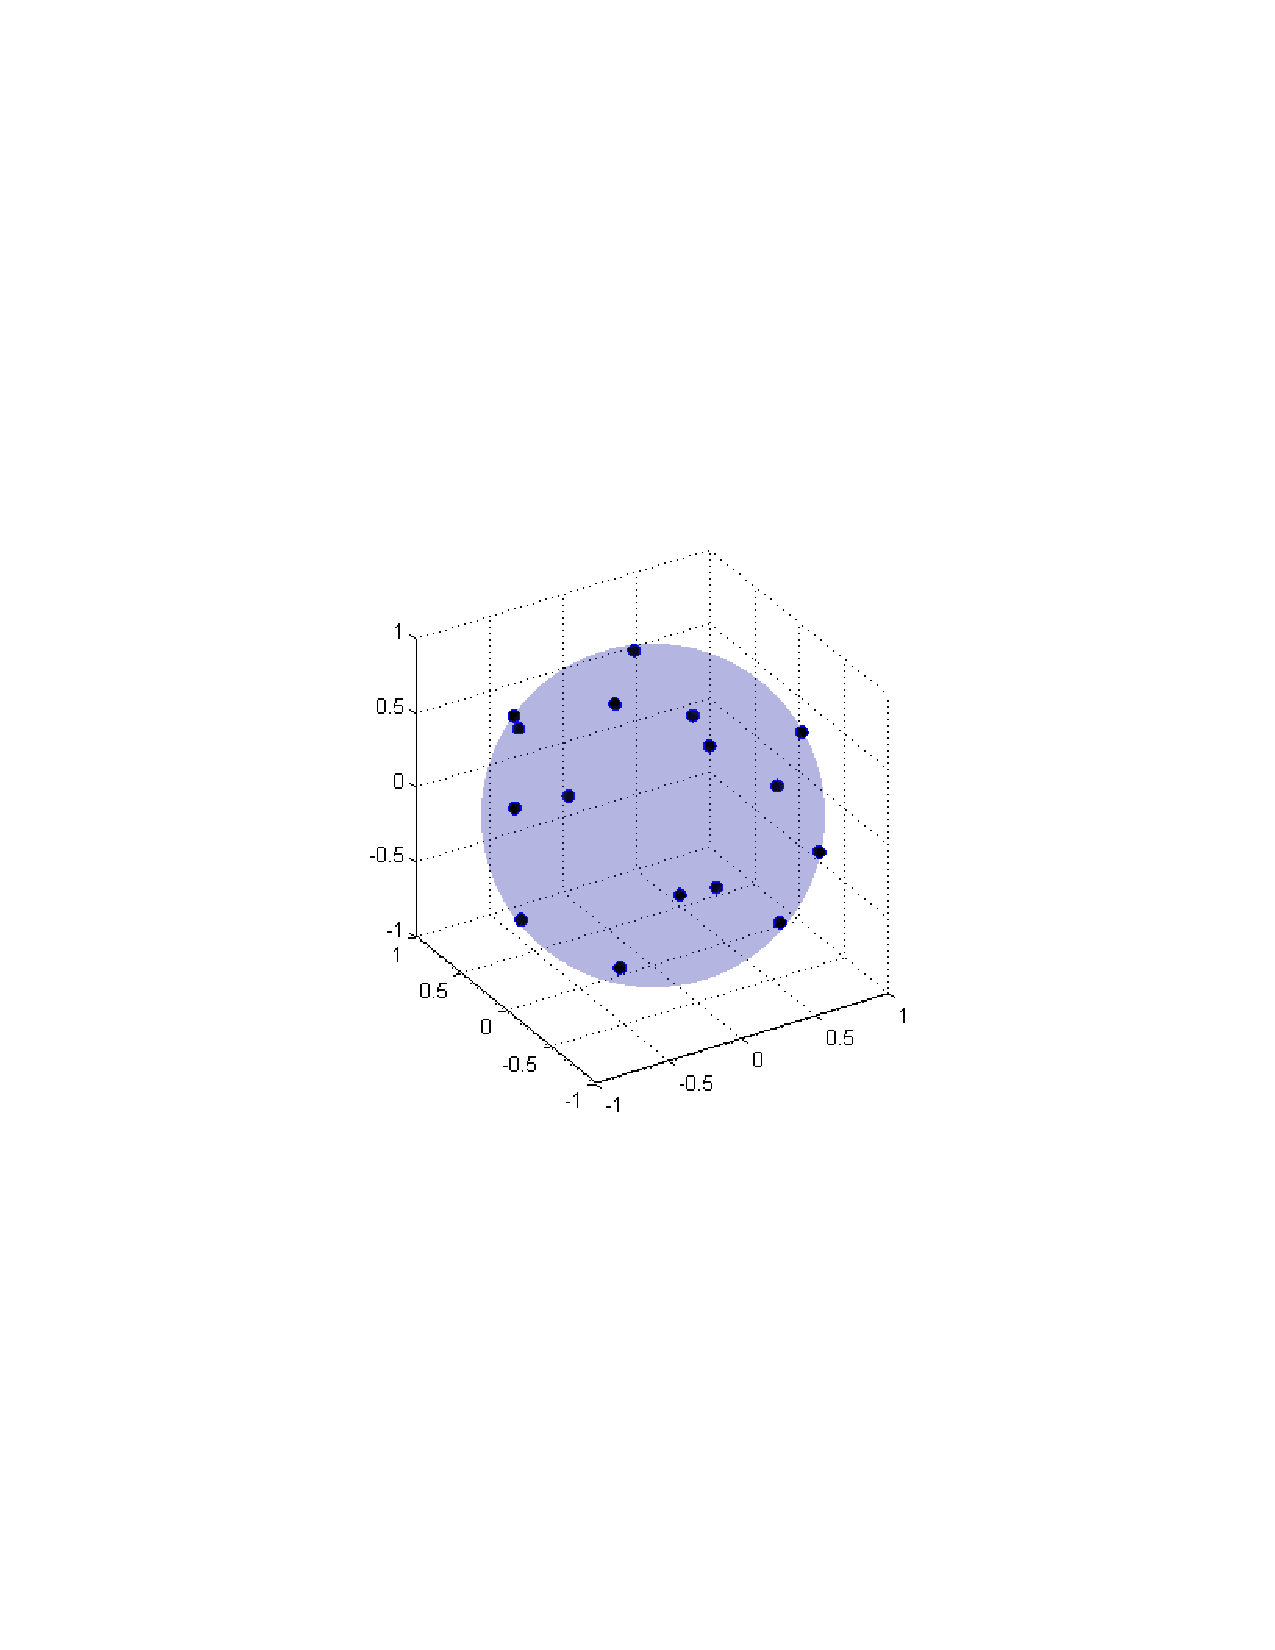
\includegraphics[width=0.5\linewidth]{images/matlab/cameras.pdf}
\caption{Positions of the first 16 cameras generated using Halton points on a sphere.}
\label{fig:cameras}
\end{figure} 

\subsubsection{Exponentially biased points}
\label{sec:exponentiallybiased}

\begin{figure}[!ht]
\centering
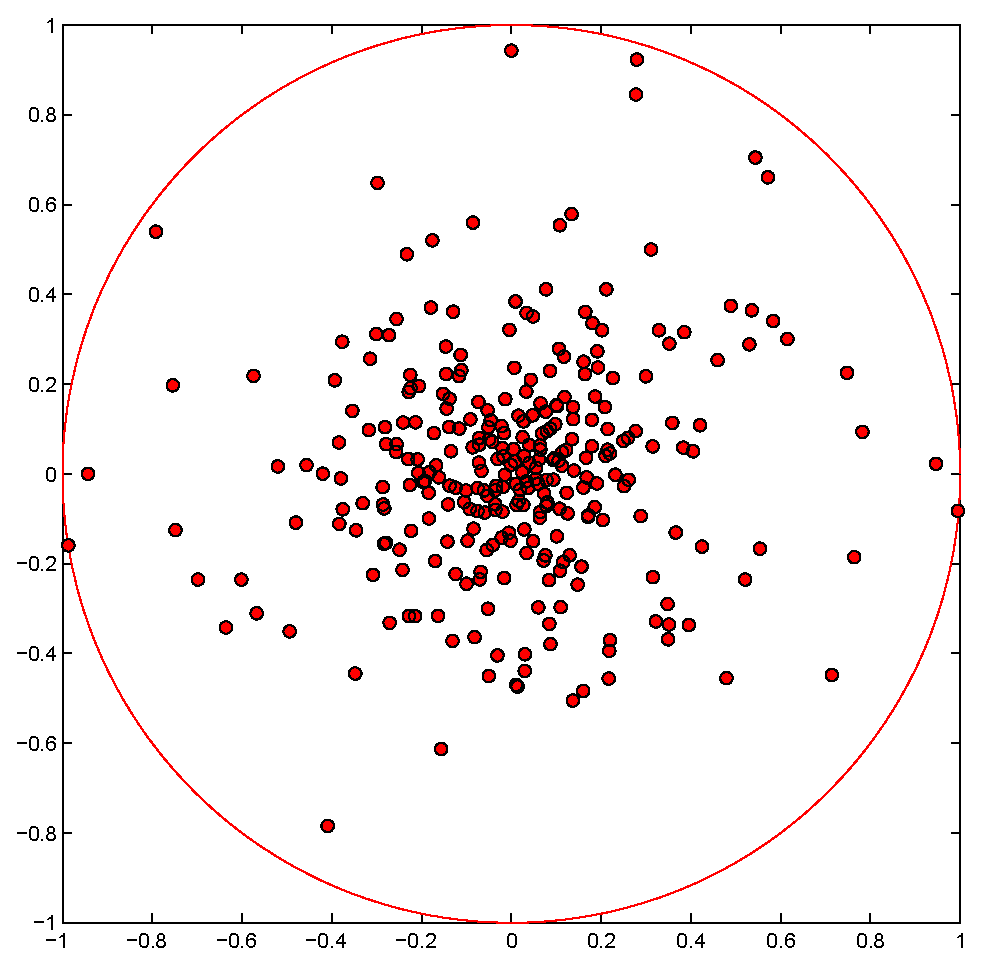
\includegraphics[width=0.7\linewidth]{images/matlab/halton_exp.eps}
\caption{Exponentially biased Halton points on a disk. The maximum radius is 1, and $M = 300$.}
\label{fig:hp}
\end{figure} 

In our algorithm, in order to obtain a better sampling, we need to have an exponentially biased distribution of points, as described in Section \ref{sec:patterns}. To obtain the disc, we employ a technique called rejection sampling. The general idea is to generate a the sequence of Halton points, then calculate their radius $r$ and calculate its probability distribution function using $\sigma_{tr}$. Then, we use the following acceptance criterion:
$$
e^{-\sigma_{tr} r} > \zeta
$$
Where $\zeta \in [0,1)$ is a pseudo-randomly generated number. We can see that if the point is close to the center ($r \rightarrow 0$), $e^{-\sigma_{tr} r} \approx 1$ and so the point is more probable to be accepted. On the other hand, if the point is far from the center of the disc ($r \rightarrow +\infty$), $e^{-\sigma_{tr} r} \approx 0$ and so the point is less probable to be accepted. The code for generating a vector of accepted points is reported in listing \ref{lst:randomexp}.

\begin{lstlisting}[language=C++,label=lst:randomexp,caption={Generation by rejection of a exponentially distributed disc. The function generates $M$ points with distribution $e^{-\sigma_{tr} r}$, and where \gl{radius} is the maximum final radius of the points.}]
void planeHaltonCircleRejectionExponential(std::vector<Vec2f> &result, int m, float sigma_tr, float radius)
{
   uint accepted = 0;

   gel_srand(0); // Setting the seed of the random number
   int i = 1;
   while(accepted < m)
   {
        Vec2f point = haltonPointCircle(i, 2, 3);
        float rad = point.length() * radius;
        float expon = exp(-sigma_tr * rad);
        float zeta = gel_rand() / ((float)(GEL_RAND_MAX));
        if(zeta < expon)
        {
            result.push_back(radius * point);
            accepted++;
        }
        i++;
   }
}
\end{lstlisting}

In our algorithm, we generate a number of samples $M$ that is fixed, with a radius equal to the size of the bounding box of the model. Then in the actual calculation only the $N$ points closest to $\x_o$ are actually used, allowing us to tweak the performance and the result. Moreover, the value of the exponent we pass to this method is not the true $\sigma_{tr}$. We pass a modified $\sigma_{tr}^*$ according to the formula:
$$
\sigma_{tr}^* = \frac{\sigma_{tr}}{q}
$$
Where $q$ is a parameter tweakable from the user. The idea is that the user can modify the distribution of the points, making them span a wider area (that is for $q > 1$) without increasing the number of samples $N$. In fact, a bigger $N$ implies a worse performance, while a bigger $q$ requires only to recompute the points. We will discuss the results for varying values of $q$ in Chapter \ref{chap:results}. 

\subsection{Shadow mapping}
\label{sec:shadow_map}
Shadow mapping is a common technique used in modern real-time graphics \citep{everitt,Segal:1992:FSL:142920.134071,williams1978a}. The idea behind it is to render an object from a light's point of view, and then use the generated depth information in order to decide if a point is shadowed or not. First of all, we convert the point into the light camera space, using a special space conversion matrix. After this, if we have a point $\mathbf{p} = (p_x,p_y,p_z)$, we compare $p_z$ to the texture $T$ sampled in the point $(p_x,p_y)$:
$$
p_z > T(p_x,p_y)
\label{eq:shadowtest}
$$ 
\begin{figure}[!ht]
\centering
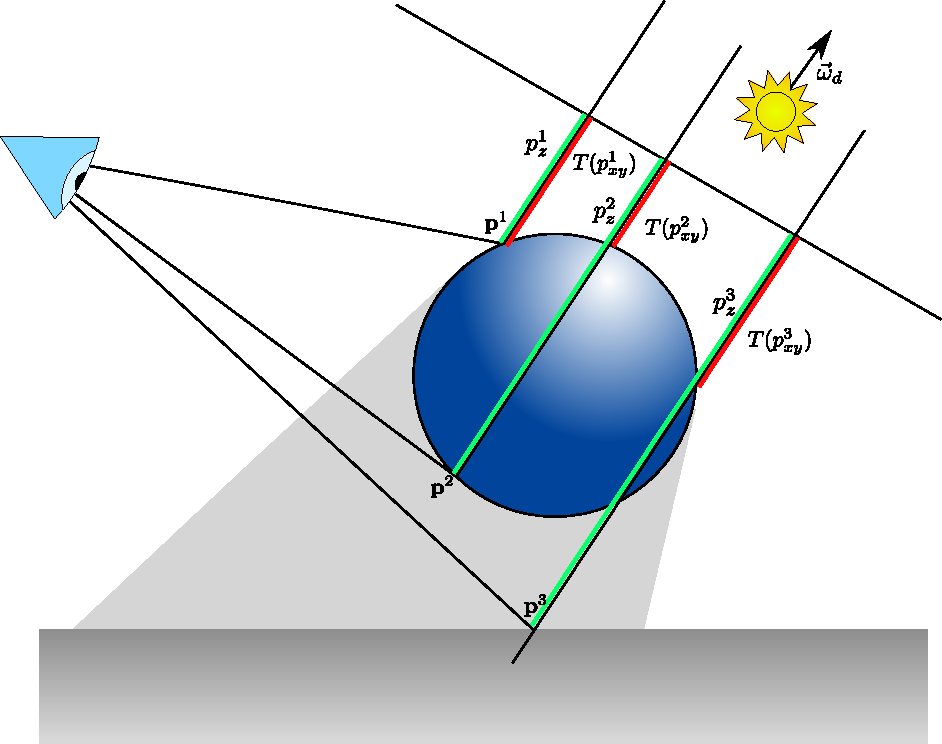
\includegraphics[width=\linewidth]{images/method/shadow_map.pdf}
\caption{Shadow mapping. We see the different results for three points $\mathbf{p^1}$, $\mathbf{p^2}$ and $\mathbf{p^3}$. The red length represents the value sampled from the depth texture($T(p_x,p_y)$), while the green length represents the value we compare against ($p_z$). When $p_z$ is less than $T(P_{xy})$, as in $\mathbf{p_1}$, the point is not shadowed. In the other cases, $\mathbf{p_2}$ and $\mathbf{p_3}$, $p_z > T(P_{xy})$and the point is not visible.}
\label{fig:shadow_map}
\end{figure} 

If the above condition is verified, it means that the current point is beneath the point visible from the light and then it should be shadowed. The matrix $L$ used to convert a point from world space to texture space is the following, using the matrix definitions and notation in Section \ref{sec:matrices}:
$$
L = T\left(\frac{1}{2}\right) \cdot S\left(\frac{1}{2}\right) \cdot P \cdot V
$$
where $P$ and $V$ are the projection and view matrix we use to render with the light. The first two matrices are necessary to convert between clip and texture coordinates, as clip coordinates are in the range $[-1,1] \times [-1,1]$, while texture coordinates are in the range $[0,1]\times[0,1]$. The process is illustrated in Figure \ref{fig:shadow_map}.

In our algorithm, we use the ideas behind shadow mapping in two different occasions. The first occasion is to get the points $x_i$ in step 2 from the texture generated in step 1, where we use the matrix $L$ in order to convert the world point $\x_o$ to $\x_d$, the center of the disc in texture space. 

The second occasion is in the final combination step, where we use also shadow mapping in order to compute the visibility function $V^k(\x)$, and to sample the radiance map. Technically, the "light cameras" in this case are the directional cameras from where we render the scene, but the concept is the same. We can see how we sample the shadow map in the final combination shader in the following listing:

\begin{lstlisting}[language=GLSL,caption={Sampling of the shadow map texture in step 3 of our method.}]
#version 430
uniform sampler2DArrayShadow depthMap;
uniform mat4 cameraMatrices[DIRECTIONS];

float sample_shadow_map(vec3 world_pos, int layer)
{
		vec4 light_pos = cameraMatrices[layer] * vec4(world_pos,1.0f);
    light_pos.z -= shadow_bias; //bias to avoid shadow acne
    if(light_pos.x < 0.0 || light_pos.x > 1.0) return 1.0;
    if(light_pos.y < 0.0 || light_pos.y > 1.0) return 1.0;
    return texture(depthMap,vec4(light_pos.x,light_pos.y,layer,light_pos.z)).r;
}        
[...] //shader code
\end{lstlisting}

In the above code, \gl{cameraMatrices[layer]} corresponds to the $L$ matrix. We use a special type of sampler, \gl{sampler2DArrayShadow}, that makes something more than its equivalent \gl{sampler2DArray}. The latter, in fact, accepts a \gl{vec3}, and simply retrieves the value in the texture. The former, on the other hand, accepts an extra parameter $z_{camera}$ (which is \gl{light_pos.z}), and compares it to the value stored in the depth texture $z_{tex}$, performing the test in equation \ref{eq:shadowtest}. If the depth of the point is less than the depth stored in the texture ($z_{camera} < z_{tex}$), 1 is returned as the point is closer to the directional camera, and thus visible. On the other hand, if $z_{camera} \ge z_{tex}$, it means the point is under the surface, and thus not visible, and 0 is returned.

To configure the \gl{sampler2DArrayShadow} texture, we need to specify some extra parameters during the depth texture initialization:

\begin{lstlisting}[language=C++,label=lst:textureconfshadow,caption={Configuration of a shadow map depth texture.}]
glBindTexture(GL_TEXTURE_2D_ARRAY, depthtex);
glTexParameterf(GL_TEXTURE_2D_ARRAY, GL_TEXTURE_MIN_FILTER, GL_NEAREST);
glTexParameterf(GL_TEXTURE_2D_ARRAY, GL_TEXTURE_MAG_FILTER, GL_NEAREST);
glTexParameterf(GL_TEXTURE_2D_ARRAY, GL_TEXTURE_WRAP_S, GL_CLAMP_TO_EDGE);
glTexParameterf(GL_TEXTURE_2D_ARRAY, GL_TEXTURE_WRAP_T, GL_CLAMP_TO_EDGE);
glTexParameterf(GL_TEXTURE_2D_ARRAY, GL_TEXTURE_COMPARE_MODE, GL_COMPARE_REF_TO_TEXTURE);
glTexParameterf(GL_TEXTURE_2D_ARRAY, GL_TEXTURE_COMPARE_FUNC, GL_LESS);
glTexStorage3D(	GL_TEXTURE_2D_ARRAY, 1, GL_DEPTH_COMPONENT32F, size, size, layers);
\end{lstlisting}

We can see that we specify two extra parameters: \gl{GL_TEXTURE_COMPARE_MODE}, once set to \gl{GL_COMPARE_REF_TO_TEXTURE}, means that sampling the depth texture in a shader will give a value based on the comparison between an extra value $z$ and the depth value $d$ in the texture. The second parameter \gl{GL_TEXTURE_COMPARE_FUNC} specifies how to compare the values: \gl{GL_LESS} means that 1 is returned if $z<d$, and zero is returned otherwise. 

\subsection{Memory layout}
\label{sec:memorylayout}
In this section, we briefly describe how we allocate memory in our method. The great advantage of using OpenGL 4.3 is that we can use \emph{texture views} \citep{openglspec}. Texture views are a way to create allocate storage for a texture in OpenGL, but on the opposite hand of \gl{glTexImage*D} or the \gl{glTexStorage*D} families of functions they allow to use another texture's storage space. To create a texture view, we use \gl{glTextureView}. We compare the standard way of allocating texture with our without texture view in Figure \ref{fig:textureviews}.

\begin{figure}[h]
\centering
\subfloat[{Without texture views}]{
  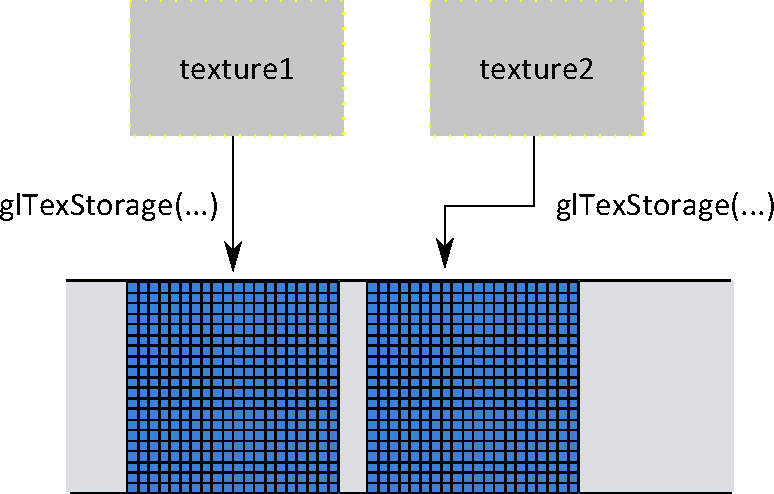
\includegraphics[width=0.5 \linewidth]{images/method/layout_no_view.pdf}
}
\subfloat[{With texture views}]{
  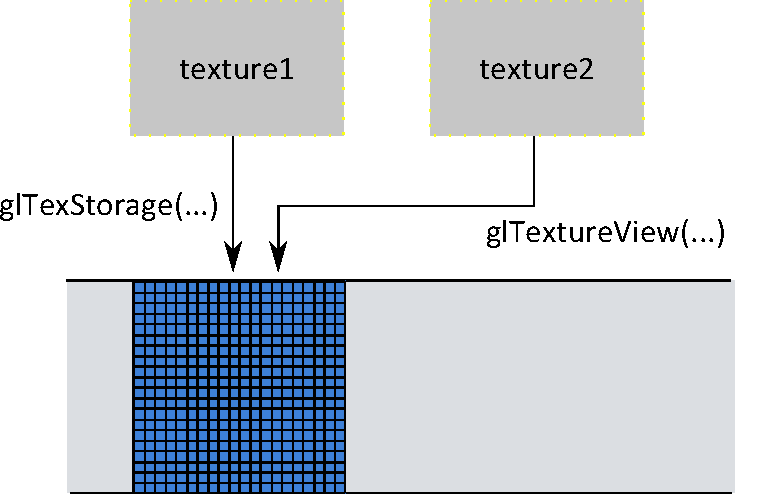
\includegraphics[width=0.5 \linewidth]{images/method/layout_view.pdf}
} 
\caption{Diagram illustrating texture views. On the top part of the picture the texture ids on the GPU, on the bottom the state of the memory. In the first case, we create two memory areas on the GPU using \gl{glTexStorage}, in the second case we make a single call to \gl{glTexStorage} and then a second call to \gl{glTextureView} to make them share the same storage space.}
\label{fig:textureviews}
\end{figure}
In our method, this comes to great advantages in two areas. First of all, since the depth texture of the radiance map is not accumulated, we can make the two radiance maps that are using ping-ponging share the same depth map. In addition, we can render directly between two mipmap levels of the same texture, something that we will need later to generate a blurred version of our texture.

A complete example memory layout for our algorithm is reported in table \ref{table:mlay}. As we will see, we will account for the contribution from multiple lights as more layers on the light map texture. More textures are loaded in order to make the method work, but their contribution to the overall memory consumption is negligible.

\begin{table}[!ht]
\centering
\begin{tabular}{p{3cm}lllll|l|}
\cline{2-7}
\multicolumn{1}{l|}{}                        & \multicolumn{1}{l|}{\textbf{Ch.}} & \multicolumn{1}{l|}{\textbf{Bits}} & \multicolumn{1}{l|}{\textbf{Width}} & \multicolumn{1}{l|}{\textbf{Height}} & \textbf{Depth} & \textbf{Size (MB)} \\ \hline
\multicolumn{1}{|l|}{Light map (vertex)}     & \multicolumn{1}{l|}{3}                 & \multicolumn{1}{l|}{32}                      & \multicolumn{1}{l|}{512}            & \multicolumn{1}{l|}{512}             & 1              & 3                  \\ \hline
\multicolumn{1}{|l|}{Light map (normals)}    & \multicolumn{1}{l|}{3}                 & \multicolumn{1}{l|}{32}                      & \multicolumn{1}{l|}{512}            & \multicolumn{1}{l|}{512}             & 1              & 3                  \\ \hline
\multicolumn{1}{|l|}{Light map (depth)}      & \multicolumn{1}{l|}{1}                 & \multicolumn{1}{l|}{32}                      & \multicolumn{1}{l|}{512}            & \multicolumn{1}{l|}{512}             & 1              & 1                  \\ \hline
\multicolumn{1}{|l|}{Radiance map 1 (color)} & \multicolumn{1}{l|}{4}                 & \multicolumn{1}{l|}{32}                      & \multicolumn{1}{l|}{512}            & \multicolumn{1}{l|}{512}             & 16             & 64                 \\ \hline
\multicolumn{1}{|l|}{Mipmaps 1}              & \multicolumn{1}{l|}{4}                 & \multicolumn{1}{l|}{32}                      & \multicolumn{1}{l|}{-}              & \multicolumn{1}{l|}{-}               & -              & 21                 \\ \hline
\multicolumn{1}{|l|}{Radiance map 2 (color)} & \multicolumn{1}{l|}{4}                 & \multicolumn{1}{l|}{32}                      & \multicolumn{1}{l|}{512}            & \multicolumn{1}{l|}{512}             & 16             & 64                 \\ \hline
\multicolumn{1}{|l|}{Mipmaps 2}              & \multicolumn{1}{l|}{4}                 & \multicolumn{1}{l|}{32}                      & \multicolumn{1}{l|}{-}              & \multicolumn{1}{l|}{-}               & -              & 21                 \\ \hline
\multicolumn{1}{|l|}{Radiance map (depth)}   & \multicolumn{1}{l|}{1}                 & \multicolumn{1}{l|}{32}                      & \multicolumn{1}{l|}{512}            & \multicolumn{1}{l|}{512}             & 16             & 16                 \\ \hline
                                             &                                        &                                              &                                     &                                      &                & \textbf{193 MB}       \\ \cline{7-7} 
\end{tabular}
\caption{Memory occupation of our method, for one light. Mipmaps are accounted for one additional third on the size of the radiance map. "Ch.` is the number of channels in the texture, "Bits` is the number of bits per channel.}
\label{table:mlay}
\end{table}

If $L$ is the number of lights, $W_l$ the size of the light map, $K$ the number of directions and $W_s$ the size of the radiance map, we can obtain a direct formula to calculate the memory consumption in bytes:
$$
4 \left\{ \left[\left(4 + 4\right) \frac{4}{3} + 1\right] K W_s^2 + \left[3 + 3 + 1\right] L W_l^2 \right\}
$$
The $4/3$ factor account for the extra space reserved for mipmaps. The 4 factor at the beginning is because each channel has 32 bits, that equal to 4 bytes. 

\FloatBarrier
\section{Caveats}
The algorithm described so far, if implemented \emph{as is}, unfortunately does not give a result that we can appreciate. In order to obtain the desired result, some extra corrections are necessary, and we are going to describe them in this section.

\subsection{Random rotation of samples}
\begin{figure}
\centering
\subfloat[Constant rotation]{
  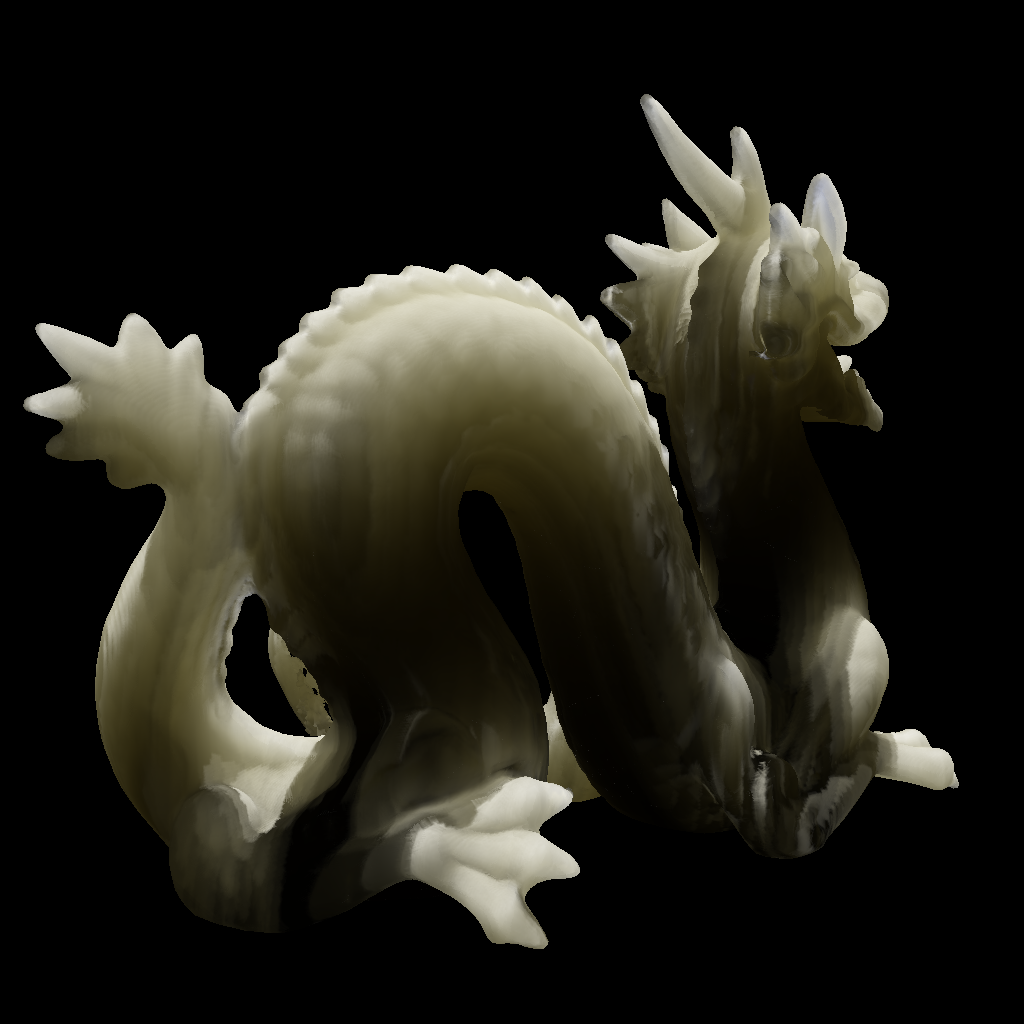
\includegraphics[width=0.5 \linewidth]{images/results/banding.png}
  \label{fig:banding1}
} 
\subfloat[Random rotation]{
  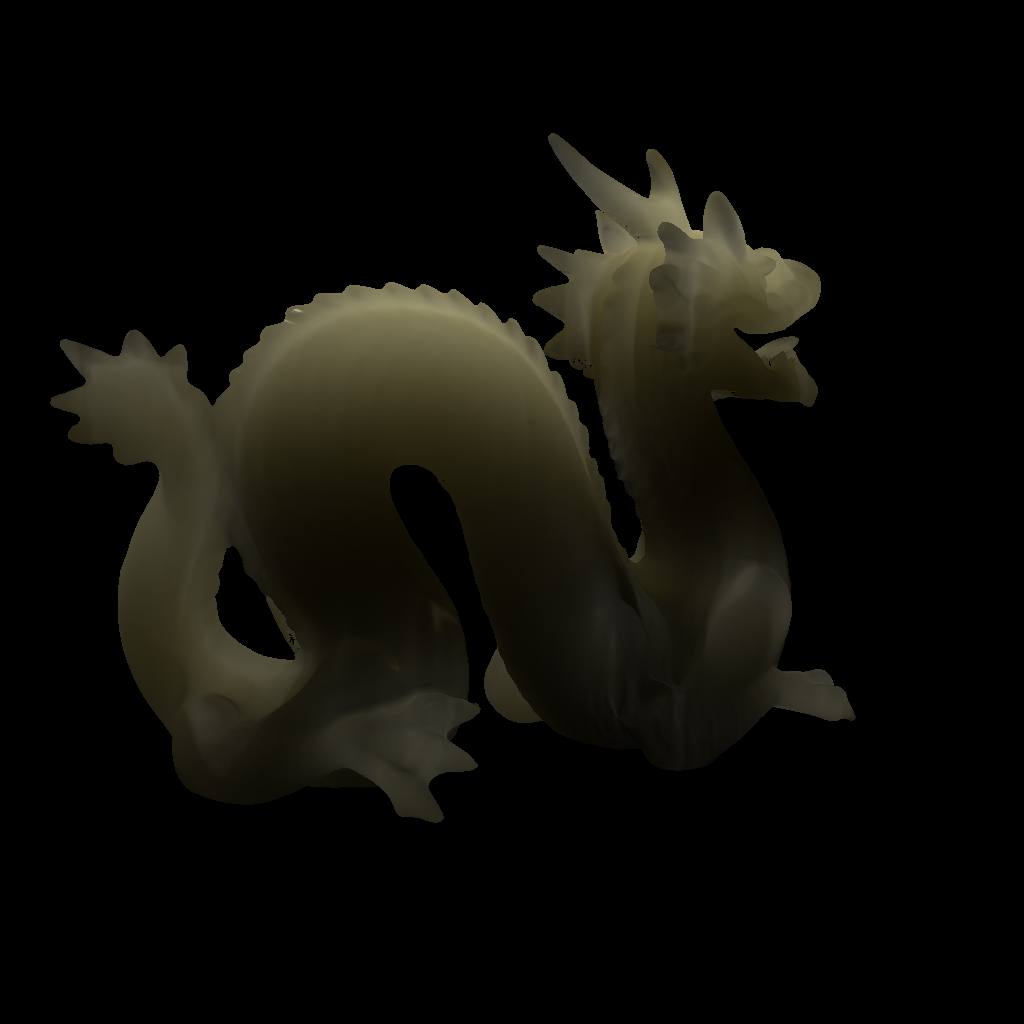
\includegraphics[width=0.5 \linewidth]{images/results/nobanding.png}
  \label{fig:banding2}
}  
\caption{White grapefruit juice dragon. The only difference in the two images is that the samples on the right figure are randomly rotated.}
\label{fig:banding}
\end{figure}

As we note in equation \ref{eq:evolution_step}, we never specified how the points in the samples are processed before actually being used in the calculation. This can lead to the assumption that the same disc pattern is used on every point $\x_o$ of the model. This causes a problem because this generates banding artifacts, as we can see in Figure \ref{fig:banding}. In order to avoid the artifacts, in exchange for noise, we randomly rotate the pattern for each pixel of the radiance map. Given that we are able to generate a random point $r$, we can take each one of the samples on the disk $\mathbf{d}_i$ and rotate it in order to obtain the new sample $\mathbf{d}_i^*$:
\renewcommand{\arraystretch}{1}
\begin{equation}
\begin{split}
\theta &= 2 \pi r \\
\mathbf{d}_i^* &= \left(\begin{array}{cc}
\cos\theta & \sin\theta \\
-\sin\theta & \cos\theta \\
\end{array} \right) \ \mathbf{d}_i
\end{split}
\label{eq:randomrot}
\end{equation}
\renewcommand{\arraystretch}{1.8}
Even if noisy, we eliminate the artifacts from the result. We will see how to reduce the noise using mipmaps in Section \ref{sec:mipmaps}. As we observed before in the overview, we also need the result to evolve on a time basis, in order not to compute the same results on every frame. Recalling that the current frame is $t$ and the maximum amount of frames before we stop the computations is $T$, we make our computation evolve using the following $\theta_t$ in equation \ref{eq:randomrot}:
$$
\theta_t = 2 \pi \left(r + \frac{t}{T}\right)
$$
This causes a progressive rotation of the disc around the point over time. However, we need still to specify how to calculate $r$. As a function, $r = (x,y,l)$ needs to depend on the fragment coordinates $(x,y)$, as well as from the current layer $l$ (to avoid two layers make the same computation). Since we are on the GPU, we cannot use a built-in random function, so we need either to load the random points from the CPU as a separate texture or to generate them on-the-fly. For the latter technique, we tried a sine based generator, a linear shift (LSR) random generator and a congruential linear generator (LCG), all in listing \ref{lst:sinegenerator}. The input point that was given was in both cases $(l \cdot x, l \cdot y)$. We can see some results in Figure \ref{fig:noises}. The sine based generator theoretically gives the best result, but the linear shift generator gives an indistinguishable result with better performance.

\begin{figure}
\centering
\subfloat[Sine noise]{
  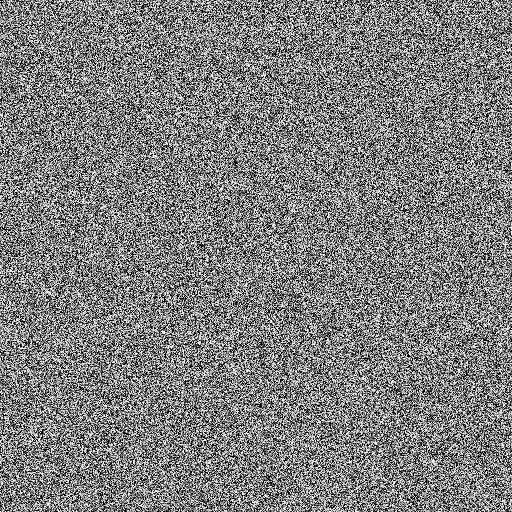
\includegraphics[width=0.33 \linewidth]{images/method/noise_1.png}
  \label{fig:noise1}
} 
\subfloat[LSR noise]{
  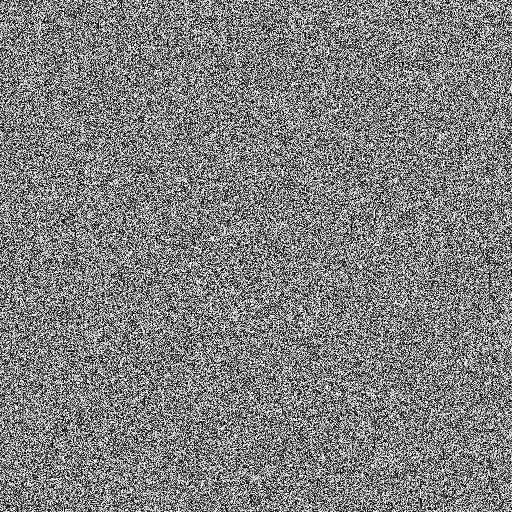
\includegraphics[width=0.33 \linewidth]{images/method/noise_2.png}
  \label{fig:noise2}
} 
\subfloat[LCG noise]{
  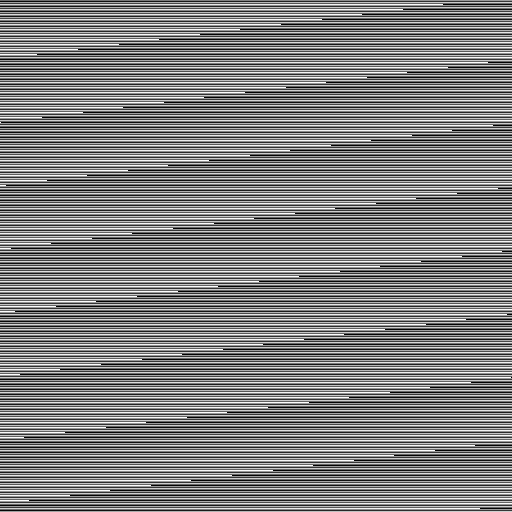
\includegraphics[width=0.33 \linewidth]{images/method/noise_3.png}
  \label{fig:noise3}
}  
\caption{Three examples of deterministic noise generation on GPU. While the sine and linear shift noises give a uniform and pleasant noise, the linear congruential generator has a periodicity.}
\label{fig:noises}
\end{figure}

\begin{lstlisting}[language=GLSL,label=lst:sinegenerator,caption={Three GLSL functions to generate random points on the GPU. The extra size parameter is the height of one layer of the radiance map texture.}]
highp float noise_sine(vec2 co)
{
    highp float a = 12.9898;
    highp float b = 78.233;
    highp float c = 43758.5453;
    highp float dt = dot(co.xy,vec2(a,b));
    highp float sn = mod(dt,3.14);
    return fract(sin(sn) * c);
}

highp float noise_lsrg(vec2 co, int size)
{
		int n = co.x + size * co.y;
    n = (n << 13) ^ n;
		int s = (n * (n*n*15731+789221) + 1376312589) & 0x7fffffff;
		return s / (4294967296.0f) * 2;
}

highp float noise_lcg(vec2 co, int size)
{
		int n = co.x + size * co.y;
		return float((n * 1664525 + 1013904223) % 4294967295) / 4294967296.0f;
}
\end{lstlisting}

\FloatBarrier
\subsection{Mipmap generation}
\label{sec:mipmaps}
The randomization we performed in the previous step comes with a drawback, i.e. we increase the noisiness of the result, especially in the initial steps. Once we reach convergence, the noisiness slowly disappears. In order to improve our method, we need to introduce a way to take the intermediate result and make it as close as possible to the final result at convergence. Our approach was to use a filter to blur the result multiple times, storing the results in the mipmaps of the radiance map generated in step 2 of our method. This results in an additional step between step 2 and step 3, where the mipmaps are calculated.

The filter that gave us the most promising results is the bilinear filter with the shape shown in Figure \ref{fig:filters}. The filter uses the alpha value of the texture as a weight for the sampled color, so the filter maintain the edges of the texture. %if time --> We can see in Figure TODO a comparison between the standard mipmap filter (which is an averaging of four neighbouring pixels) and our bilinear filter, noticing immediately the result.

\begin{figure}[!h]
\centering
\subfloat{
  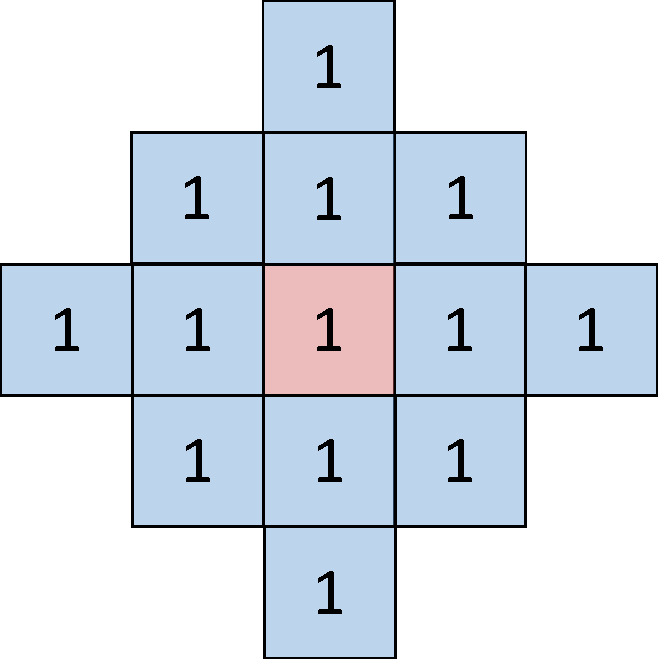
\includegraphics[width=0.33 \linewidth]{images/method/filter_1.pdf}
  \label{fig:filter1}
} 
\subfloat{
  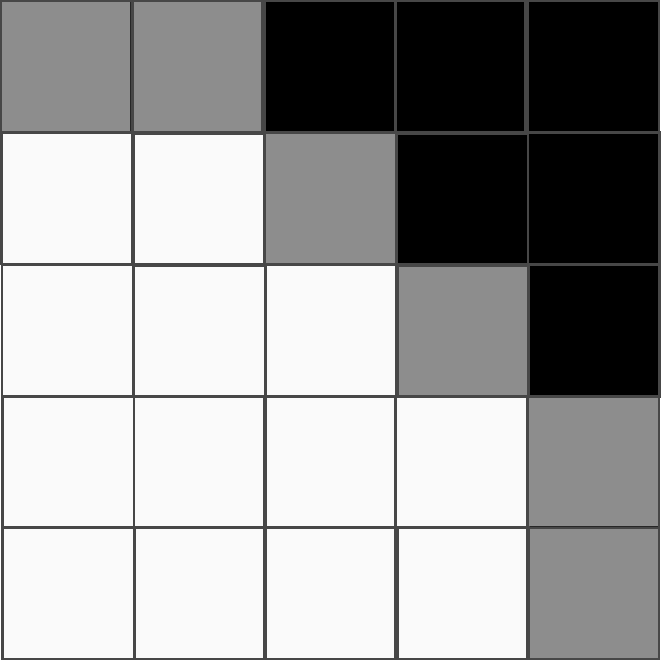
\includegraphics[width=0.33 \linewidth]{images/method/filter_2.pdf}
  \label{fig:filter2}
} 
\subfloat{
  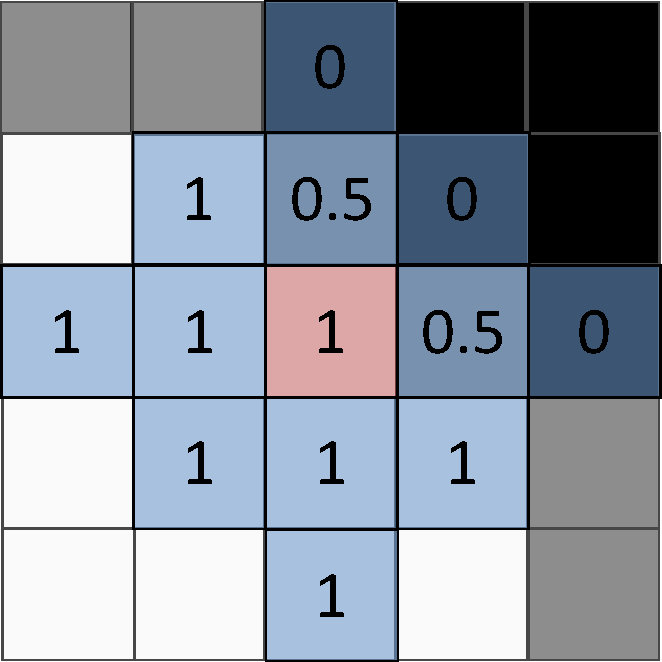
\includegraphics[width=0.33 \linewidth]{images/method/filter_3.pdf}
  \label{fig:filter3}
}  
\caption{Alpha-weighted bilinear filter. In \ref{fig:filter1} we have the shape of the filter. In \ref{fig:filter2} we have the alpha channel of an example image, to which we show the weights used in the filters in Figure \ref{fig:filter3}, based on the alpha channel of the picture.}
\label{fig:filters}
\end{figure}

On the implementation level, the mipmaps need to be rendered one after the other, as we need the result of the first computation in order to perform the second. So, we use always the same shader, reported in listing \ref{lst:shaderimageprocessing}, to filter between two textures. In the first step, we bind layer zero (where the result of the rendering of step 2 is stored) as source and layer 1 as destination. Then, we bind layer 1 as source and layer 2 as destination, and so on. To perform the filtering, we render a full screen quad.

However, OpenGL does not allow to bind the same image both as a source and as a destination, even if the mipmap levels are different. So, in order to overcome this difficulty, we use texture views as we described them in \ref{sec:memorylayout}. We create a new texture for the mipmaps, but then we configure it to use the storage reserved to the mipmaps of the radiance map. So, we can bind it to the FBO as it was a completely different texture, but then once we render the result will be rendered in the right memory location. 

\begin{lstlisting}[language=GLSL,label=lst:shaderimageprocessing,caption={Custom mipmap filtering on GPU. \gl{_tex} are the texture coordinates on the screen aligned quad.}]
#version 430
in vec3 _tex;
uniform sampler2DArray source;

out vec4 fragColor;

uniform float texStep;
uniform int scaling;

void main(void)
{
	int layer = gl_Layer;
	float t_step = texStep * 0.5 * scaling;
	vec4 c0  = texture(source,vec3(_tex.xy,layer));
	vec4 c1  = texture(source,vec3(_tex.xy + vec2(t_step,0.0f),layer));
	vec4 c2  = texture(source,vec3(_tex.xy - vec2(t_step,0.0f),layer));
	vec4 c3  = texture(source,vec3(_tex.xy + vec2(0.0f, t_step),layer));
	vec4 c4  = texture(source,vec3(_tex.xy - vec2(0.0f, t_step),layer));

	vec4 c5  = texture(source,vec3(_tex.xy + 2 * vec2(t_step,0.0f),layer));
	vec4 c6  = texture(source,vec3(_tex.xy - 2 * vec2(t_step,0.0f),layer));
	vec4 c7  = texture(source,vec3(_tex.xy + 2 * vec2(0.0f, t_step),layer));
	vec4 c8  = texture(source,vec3(_tex.xy - 2 * vec2(0.0f, t_step),layer));

	vec4 c9  = texture(source,vec3(_tex.xy + vec2(t_step,t_step),layer));
	vec4 c10 = texture(source,vec3(_tex.xy - vec2(t_step,t_step),layer));
	vec4 c11 = texture(source,vec3(_tex.xy + vec2(t_step, -t_step),layer));
	vec4 c12 = texture(source,vec3(_tex.xy - vec2(t_step, -t_step),layer));

	float v0 = clamp(c0.a,0.0f,1.0f);
	float v1 = clamp(c1.a,0.0f,1.0f);
	[...] //omitted
	float v12 = clamp(c12.a,0.0f,1.0f);

	vec4 step1 = c0 * v0 + c1 * v1 + c2 * v2 + c3 * v3 + c4 * v4;
	float vstep1 = v0 + v1 + v2 + v3 + v4;
	vec4 step2 = c5 * v5 + c6 * v6 + c7* v7 + c8 * v8;
	float vstep2 = v5 + v6 + v7 + v8;
	vec4 step3 = c9 * v9 + c10 * v10 + c11 * v11 + c12 * v12;
	float vstep3 = v9 + v10 + v11 + v12;

	fragColor = (step1 + step2 + step3 )/max(vstep1 + vstep2 + vstep3, 1.0f);
}
\end{lstlisting}

\begin{figure}[!h]
\centering
\subfloat{
  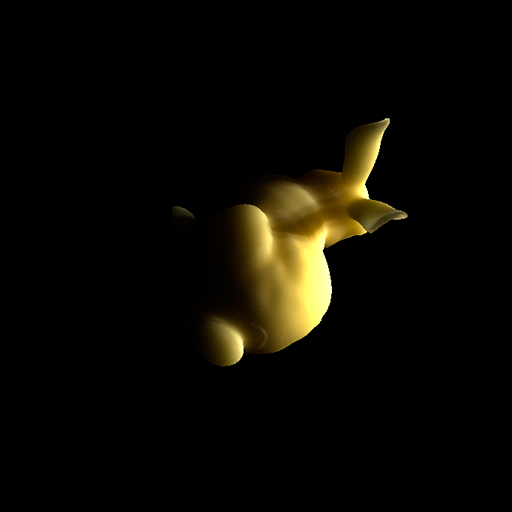
\includegraphics[width=0.33 \linewidth]{images/results/mipmap_0.png}
  \label{fig:mip0}
} 
\subfloat{
  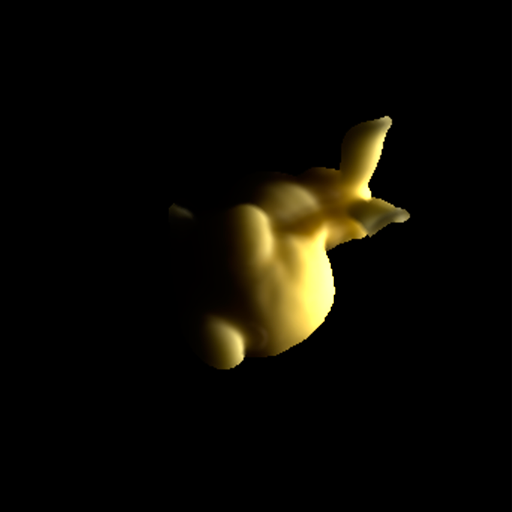
\includegraphics[width=0.33 \linewidth]{images/results/mipmap_1.png}
  \label{fig:mip1}
} 
\subfloat{
  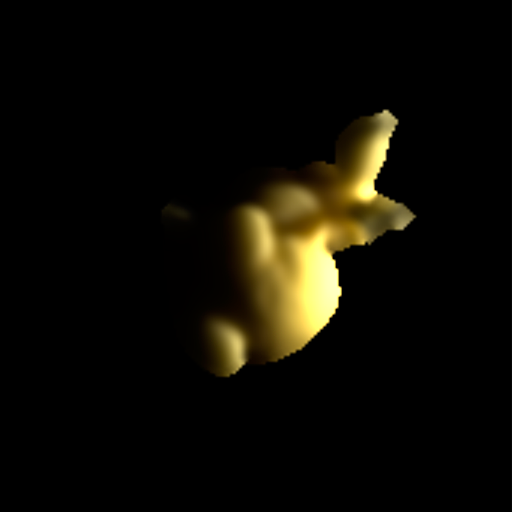
\includegraphics[width=0.33 \linewidth]{images/results/mipmap_2.png}
  \label{fig:mip2}
}  \\
\subfloat{
  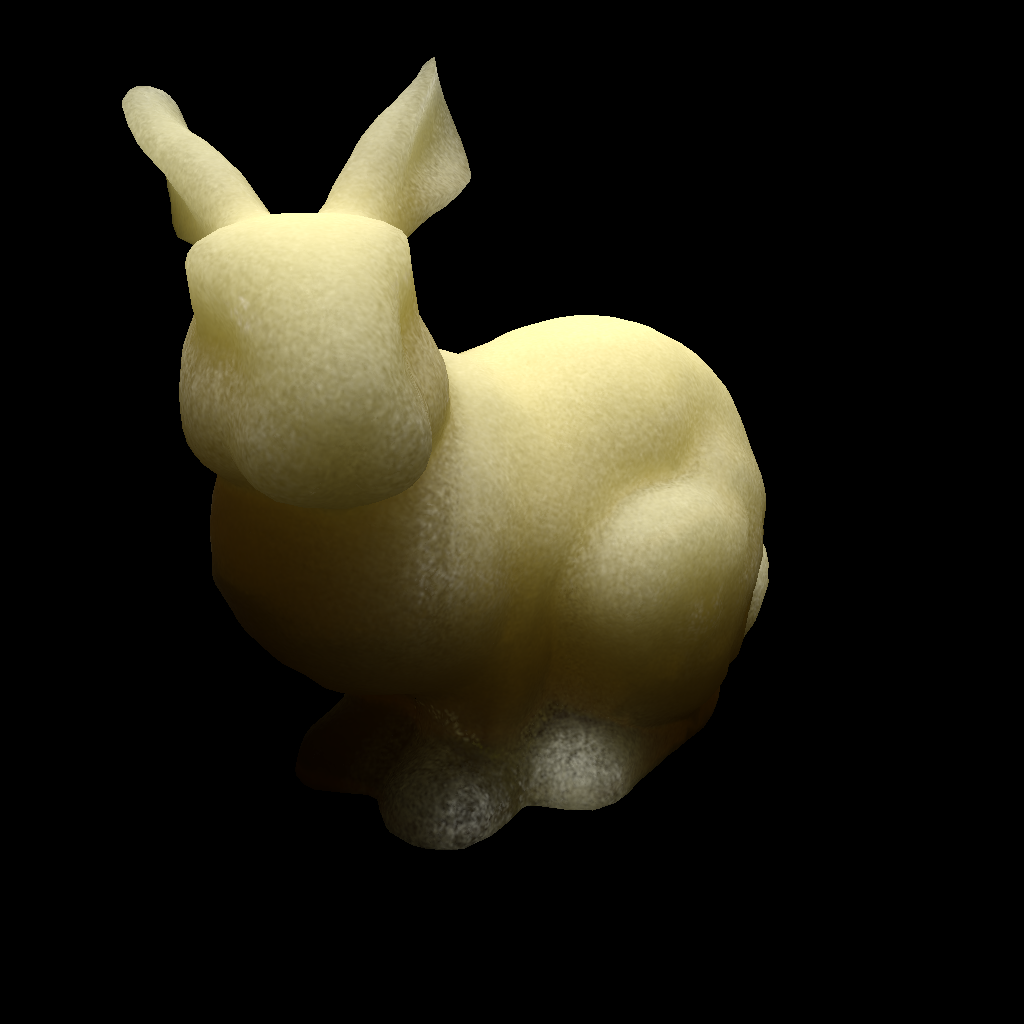
\includegraphics[width=0.33 \linewidth]{images/results/jeppe_noise.png}
  \label{fig:jenoise}
} 
\subfloat{
  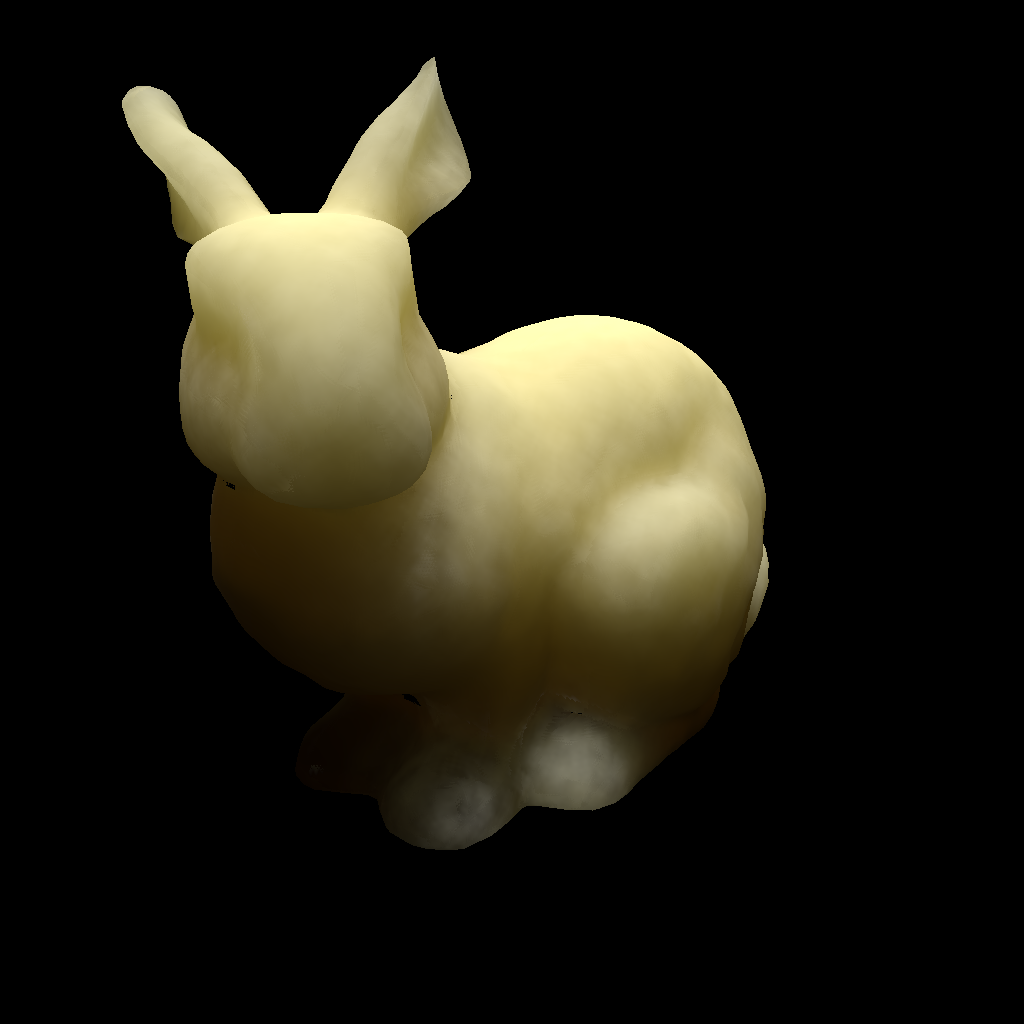
\includegraphics[width=0.33 \linewidth]{images/results/jeppe_mipmap_1.png}
  \label{fig:jemip1}
} 
\subfloat{
  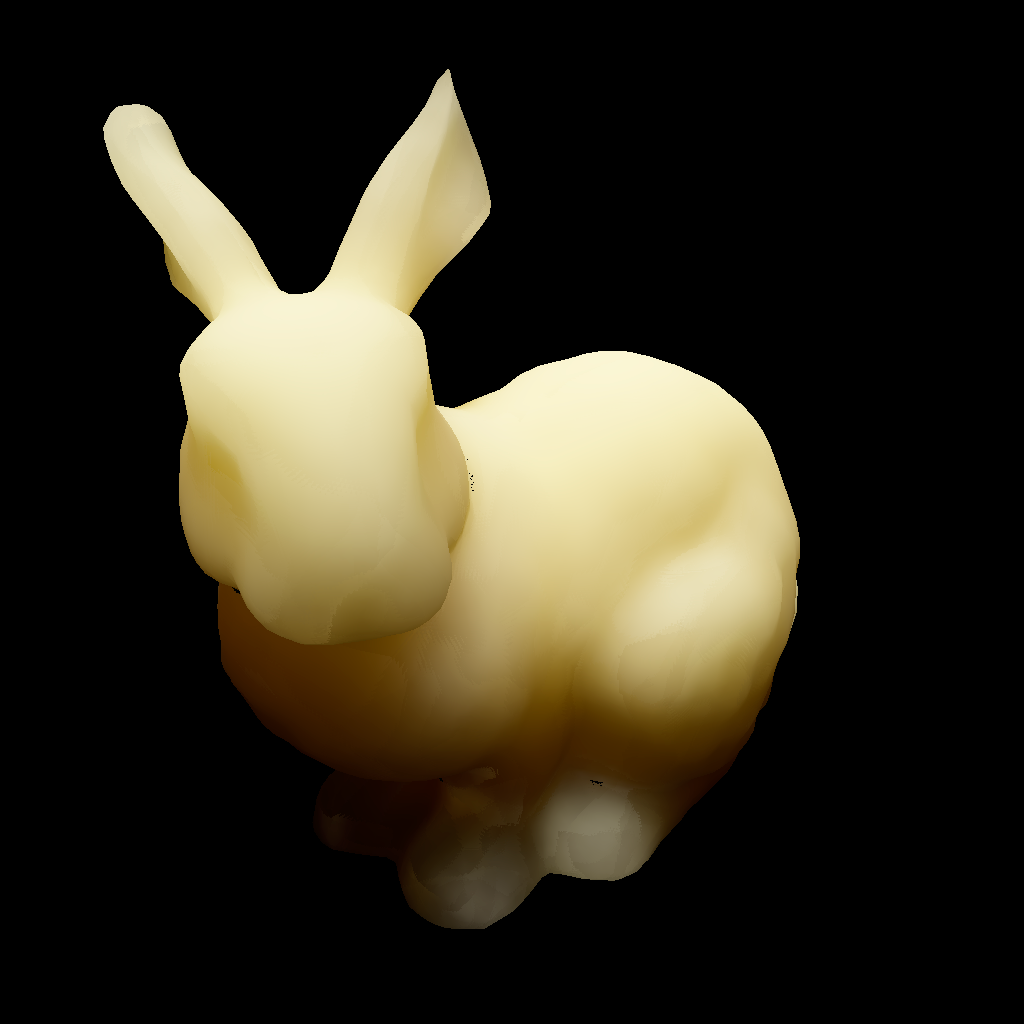
\includegraphics[width=0.33 \linewidth]{images/results/jeppe_mipmap_2.png}
  \label{fig:jemip2}
}  
\caption{Mipmap generation. On the first row, left to right, the base level and two subsequent applications of the bilinear filter (the images have been cropped for a better visualization). On the bottom row, the model sampled with the different mipmap levels. We note that at level 2 artifacts start to emerge along the camera seams.}
\label{fig:mipmaps}
\end{figure}

\FloatBarrier
\subsection{Shadow bias}

The shadow mapping described in Section \ref{sec:shadow_map} has an obvious problem, called \emph{shadow acne}. As we can see in Figure \ref{fig:shadowbias}, the discretization of depth comes with a problem: depending on the incidence angle, the surface starts generating an alternating pattern of dark and light on the visible areas. The solution in this case is to introduce a constant factor when we are comparing the texture space position and the depth of a point, called \emph{shadow bias} $\epsilon_b$. The test then becomes:
$$
p_z - \epsilon_b < T(p_x,p_y)
$$ 
The result is depicted in Figure \ref{fig:shadowbias}. As we can see, we raise the sampling by the bias factor, so the lit areas do not present shadow acne anymore. This comes with a drawback: the shadow bias, for thin objects, it introduces another artifact, called \emph{peter panning}, i.e. the shadow and the object become disconnected. In the case of our method, a too large bias makes the different directions to become "disconnected", not representing a faithful result. 

\begin{figure}[!h]
\centering
\subfloat[Shadow acne]{
  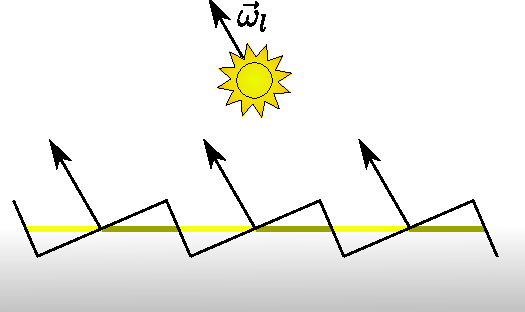
\includegraphics[width=0.5 \linewidth]{images/method/shadow_bias.pdf}
  \label{fig:acne}
}
\subfloat[Shadow acne, with shadow bias]{
  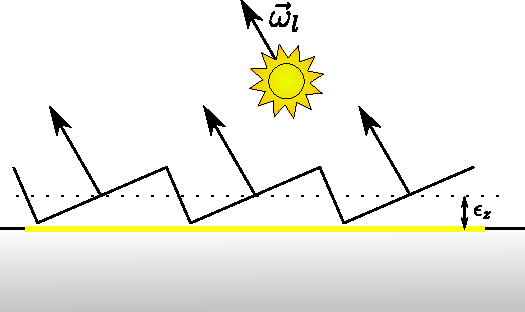
\includegraphics[width=0.5 \linewidth]{images/method/shadow_bias_correct.pdf}
  \label{fig:bias}
} \\
\subfloat[Shadow acne, result]{
  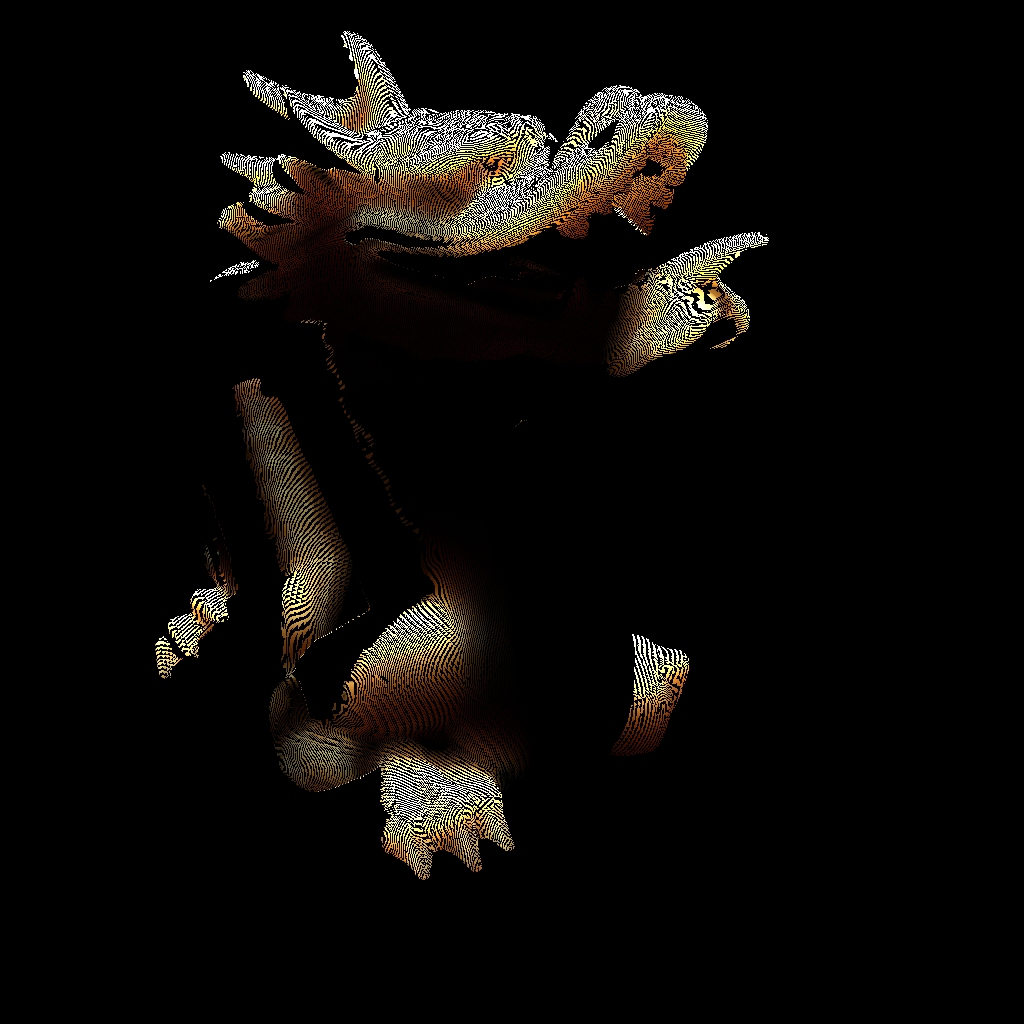
\includegraphics[width=0.5 \linewidth]{images/method/acne.png}
  \label{fig:acneres}
}
\subfloat[Shadow acne, with shadow bias, result]{
  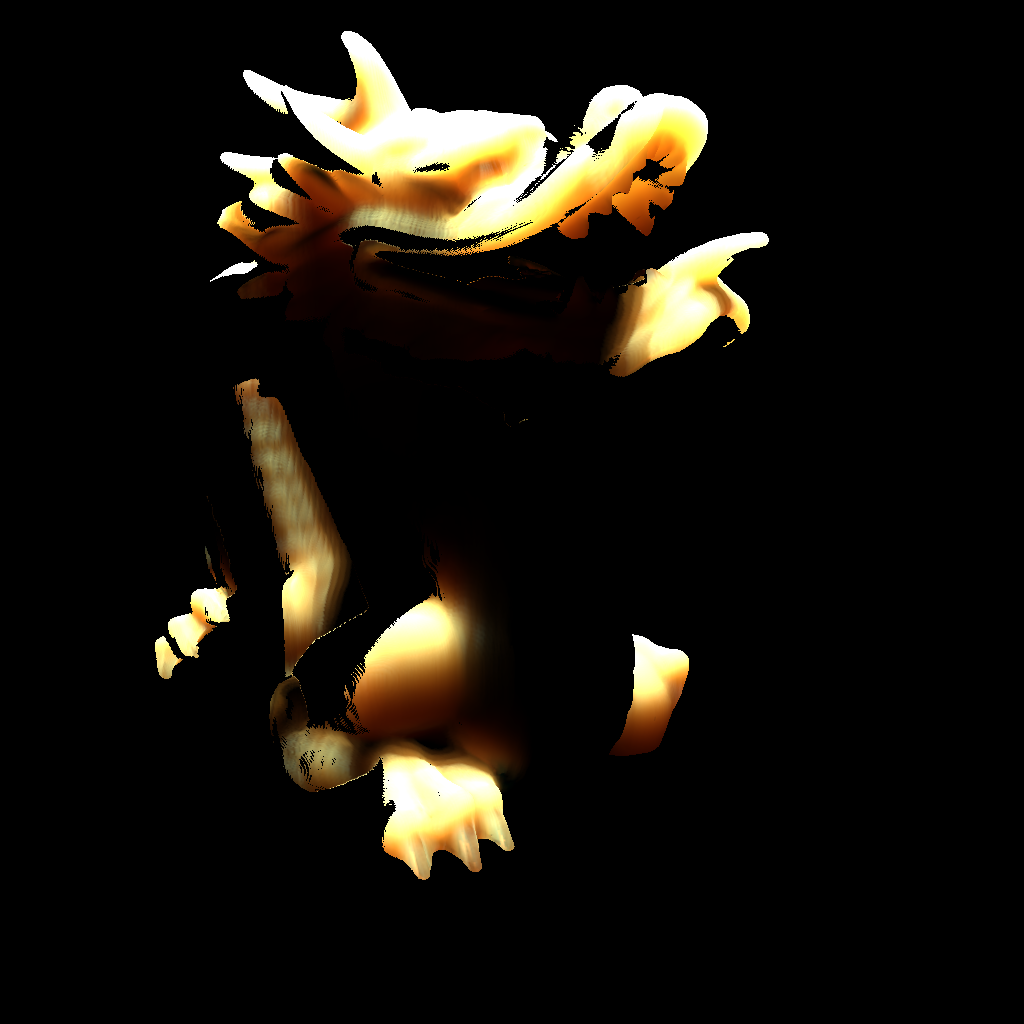
\includegraphics[width=0.5 \linewidth]{images/method/noacne.png}
  \label{fig:biasres}
}

\caption{Shadow acne (Figure \ref{fig:acne}) origin: the angle of the light causes little bands to appear. Adding a small offset $\epsilon_z$ to the sampling (\ref{fig:bias}) corrects the result, leading to a full lit surface. On the bottom row, the two figures \ref{fig:acneres} and \ref{fig:biasres} show the results with and without the correction.}
\label{fig:shadowbias}
\end{figure}

\FloatBarrier
\subsection{Texture discretization artifacts}
A problem related to the previous one is texture discretization artifacts, that appear as seams in the texture in Figure \ref{fig:combias}. The problem is similar to the one of depth bias, but it manifests on the direction perpendicular to the directional cameras. Because of the discretization and the depth bias in the shadow sampling, some pixels become false positives, being incorrectly sampled even if they are not visible. To fix this, we apply a transformation to the vertex in the final step that shrinks it a little bit towards the center of the texture. The shrinking is made using the camera direction as a main axis, according to the formula:
$$
\x_o^{shrink} = \x_o - \epsilon_c (\vec{n}_o - \vomega_d (\vec{n}_o \cdot \vomega_d));
$$
Where $\epsilon_c$ is a parameters set by the user. In this way we obtain a shrinkage of one pixel of the model when we use $\x_o^{shrink}$ for sampling the radiance map. As we can see in Figure \ref{fig:combias}, adding this correction solves the problem.

\begin{figure}
\centering
\subfloat[Without correction]{
  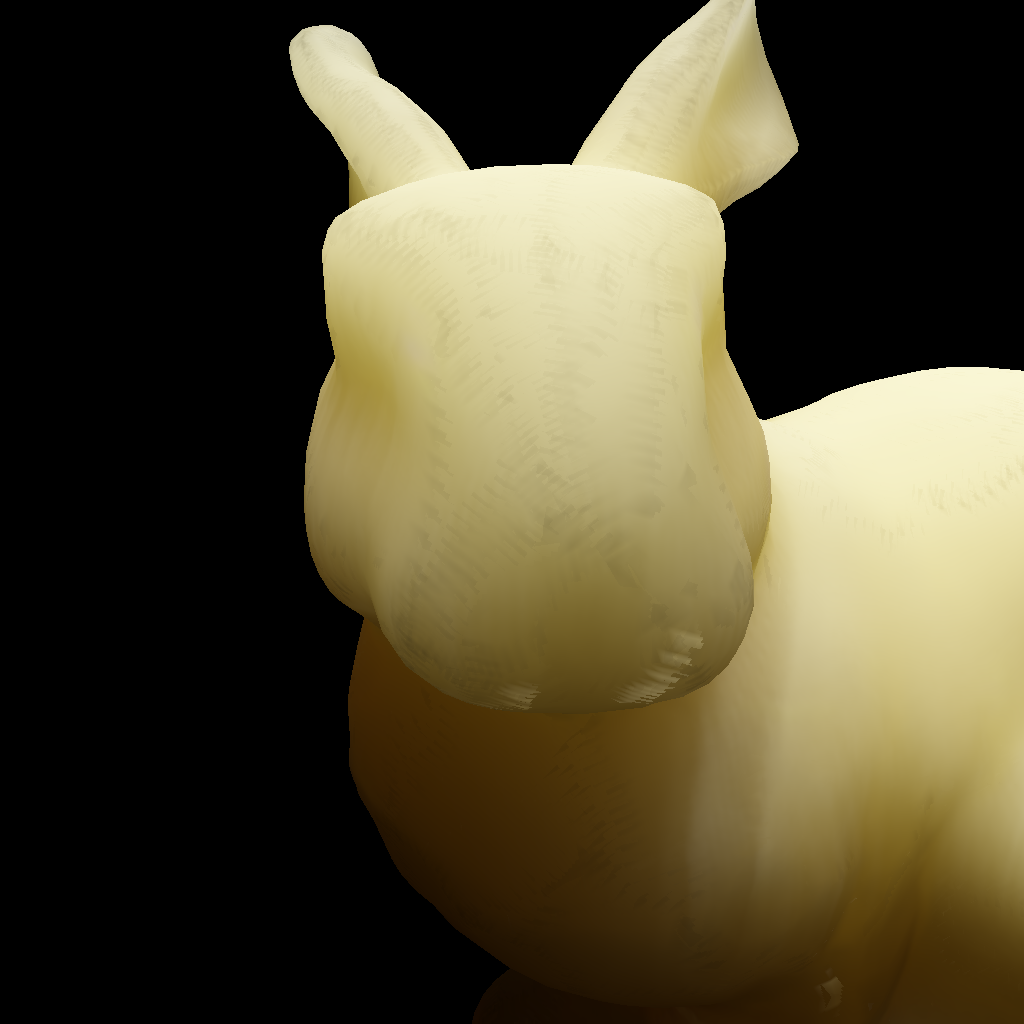
\includegraphics[width=0.5 \linewidth]{images/results/comb_offset.png}
  \label{fig:comb_off}
}
\subfloat[With correction]{
  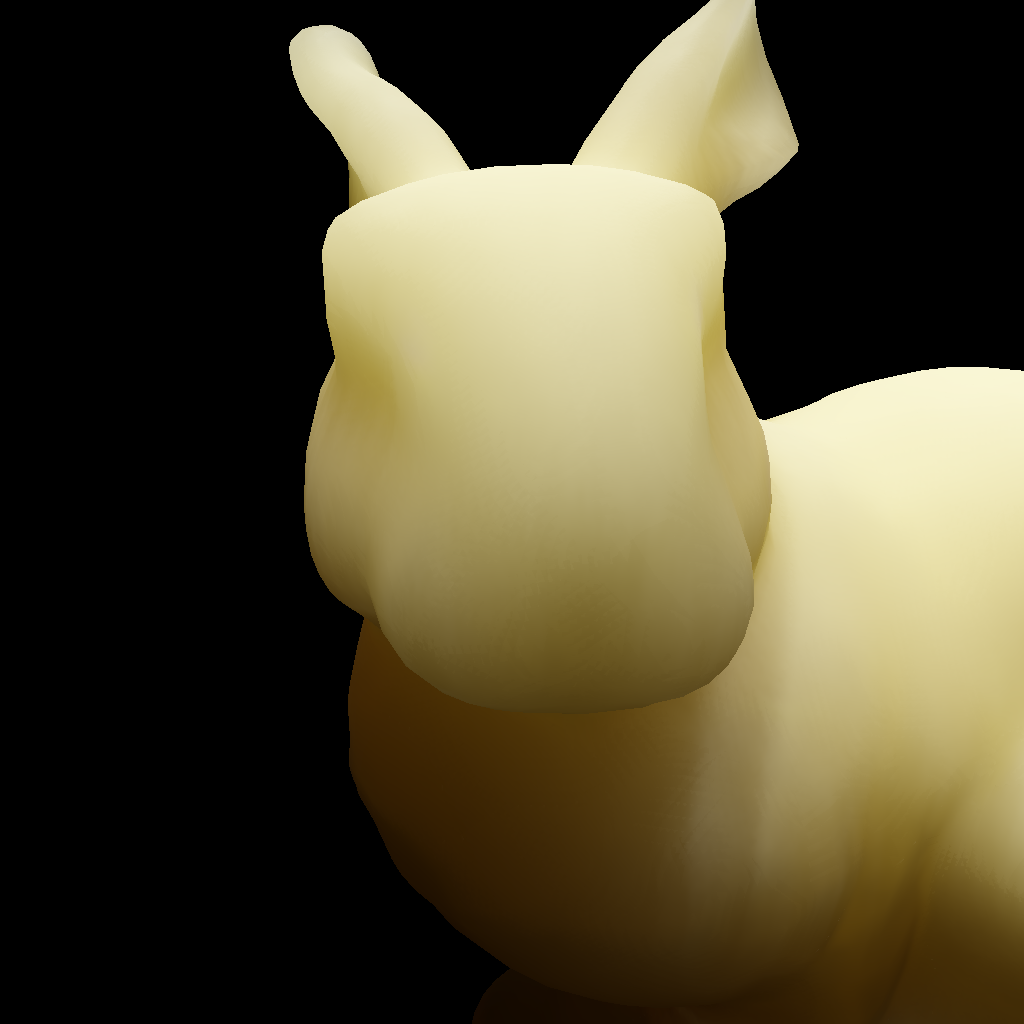
\includegraphics[width=0.5 \linewidth]{images/results/comb_offset_solved.png}
  \label{fig:comb_off_solved}
} 
\caption{Combination offset artifacts. Without the correction, artifacts start to appear. With a correction of $0.002 \approx 2 / 1024$ the result is greatly improved.}
\label{fig:combias}
\end{figure}


\section{Extensions to the method}

In this section, we describe briefly how we extended our implementation in order to cover a wider range of cases, especially regarding different types of light.

\subsection{Rendering with multiple lights}

\begin{figure}[!h]
\centering
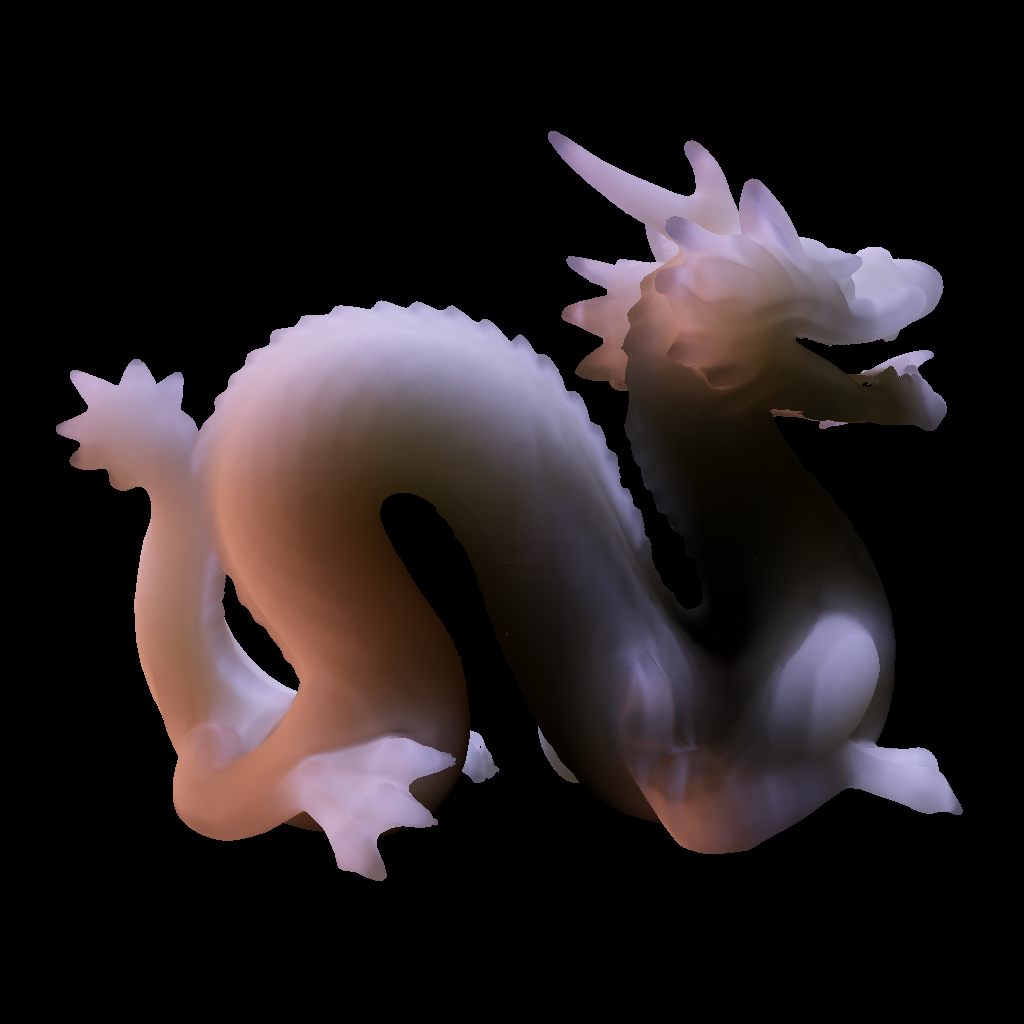
\includegraphics[width=0.9 \linewidth]{images/results/multiple.png}
\caption{Rendering with two point lights. The material parameters used are for white grapefruit juice. One light comes from the left ($\vomega_l = (1,0,0)$), with radiance $L_d = (13,5,5)$. One comes from the top ($\vomega_l = (0,0,1)$), with radiance $L_d = (5,5,13)$.}
\label{fig:multilight}
\end{figure}

Rendering with multiple lights requires only a slight extension to the method. We just need to adjust the computation in \ref{eq:evolution_step} in order to account for multiple lights, obtaining a result as the one in Figure \ref{fig:multilight}. We notice that this computation may come with a performance penalty, since we are now computing the contribution from $L N$ samples instead of $N$, where $L$ is the number of lights. To avoid this, we account in advance and calculate only $\frac{N}{L}$ samples per light:
$$
R^{t,k}(\x_o) = \sum_{l = 1}^L L_l \sum_{i = 1}^{N/L} S(\x^{t,k}_i, \vomega^t_l, \x_o, \vomega_o) \exp\left(\sigma_{tr} r^{t,k}_i\right), \ \ t \in [0,T], \ \ k \in [0,K-1] 
$$
We can see that only the light vector $\vomega^t_l$ and the radiance $L_l$ depend on the current light, while the other parameters are left unchanged. On the implementation level, we first need to change the light map in order to be a layered texture as well. As in step 2, we employ layered rendering to render all the light maps at same time. Then we simply add an extra loop in the shader of step 2 to account for multiple lights. As for the light parameters, they are passed to the shader as arrays of uniforms. The outline of the new shader illustrating how lights are computed is listed in listing \ref{lst:multi}.

\begin{lstlisting}[language=GLSL,label=lst:multi,caption={Outline of the shader in step 2 with support for multiple lights.}]
#version 430
layout(location = 0) out vec4 fragColor;

[...] // constants, includes, textures omitted

uniform sampler2DArray vtex; // texture with vertices
uniform sampler2DArray ntex; // texture with normals

smooth in vec3 position;
smooth in vec3 norm;

uniform vec4 light_pos[MAX_LIGHTS];
uniform vec4 light_diff[MAX_LIGHTS];
uniform int light_number;
uniform mat4 lightMatrices[MAX_LIGHTS];

[...] //BSSRDF code, uniform and functions

void main(void)
{
    vec3 xo = position;
    vec3 no = normalize(norm);

		[...] // sampling the old color, noise calculation

    for(int k = 0; k < light_number; k++)
    {
        vec3 wi = light_pos[k].xyz;
        vec4 light_post = lightMatrices[k] * vec4(xo,1.0f);
        vec2 circle_center = light_post.xy;
        vec3 Li = light_diff[k].xyz;
				
        for(int i = 0; i < max_samples; i++)
        {
						[...] // sampling from layer k in textures vtex and ntex
						[...] // summing over BSSRDF on vector accumulate
        }
    }

    fragColor = vec4(accumulate,1.0f);
		[...] //adding old color
}
\end{lstlisting}
\clearpage
\subsection{Rendering with other kinds of light}
Our method does not depend on a specific type of light in order to render a material. Once we have a formula for the radiance for the light, we can simply introduce it in equation \ref{eq:evolution_step} and compute the result. So, for example, for a point light the equation would become.
$$
R^{t,k}(\x_o) = {I_l} \sum_{i = 1}^N  \frac{S(\x^{t,k}_i, \frac{\x_l - \x_i}{\|\x_l - \x_i\|}, \x_o, \vomega_o)}{{\|\x_l - \x_i\|}} \exp\left(\sigma_{tr} r^{t,k}_i\right), \ \ t \in [0,T], \ \ k \in [0,K-1] 
\label{eq:evolution_step_2}
$$
Where $\x_l$ is the light position and $I_l$ the light intensity. More generally, if we have a function to compute the light direction $\vomega_l(\x_i)$ and a function to compute radiance $L(\x_i, \vomega_l(\x_i))$ we can express equation \ref{eq:evolution_step} in the following way:
$$
R^{t,k}(\x_o) = \sum_{l = 1}^L \sum_{i = 1}^{N/L} L^t(\x_i, \vomega_l(\x_i)) S(\x^{t,k}_i, \vomega_l^t(\x_i), \x_o, \vomega_o) \exp\left(\sigma_{tr} r^{t,k}_i\right)
$$
If we have only point and directional lights, we have the following setup for the two formulas:
\begin{equation*}
\begin{split}
\vomega_l(\x_i) &= \begin{cases}
\vomega_l & \text{if l is directional with $\vomega_l$, $L_l$} \\
 \frac{\x_l - \x_i}{\|\x_l - \x_i\|} & \text{if $l$ is point with $\x_l$, $I_l$}
\end{cases} \\
L(\x_i, \vomega_l(\x_i)) &= \begin{cases}
L_l & \text{if l is directional with $\vomega_l$, $L_l$} \\
 \frac{I_l}{\|\x_l - \x_i\|} & \text{if $l$ is point with $\x_l$, $I_l$}
\end{cases} \\
\end{split}
\end{equation*}
On the implementation level, we can still use same uniforms that we use for multiple lights: the position vector will become either the position of the direction of the light. We make the position vector of the light carry some extra information in the alpha channel: if the alpha is zero (i.e. the vector is of type $(x,y,z,0)$), we are dealing with a directional light, while if the alpha is one (i.e. the vector is of type $(x,y,z,1)$) we are using a point light. The code to calculate lights thus becomes:
\begin{lstlisting}[language=GLSL,label=lst:multilighttype,caption={GLSL Code to calculate the radiance \gl{Li} and the incoming light direction \gl{wi} for the k-th directional or point light source.}]
int current_light = k;
vec3 wi = light_pos[current_light].xyz;
vec4 rad = light_diff[current_light];
vec3 topoint = wi - xo;
float light_type = light_pos[current_light].a;
wi = (light_type > 0)? normalize(topoint) : normalize(wi);
vec3 Li = light_diff[current_light].xyz;
Li = (light_type > 0)? Li / dot(topoint,topoint) : Li;
\end{lstlisting}
\begin{figure}[!h]
\centering
\subfloat[Directional:  $\vomega_l = (0,0,1)$ $L_d = (8,8,8)$]{
  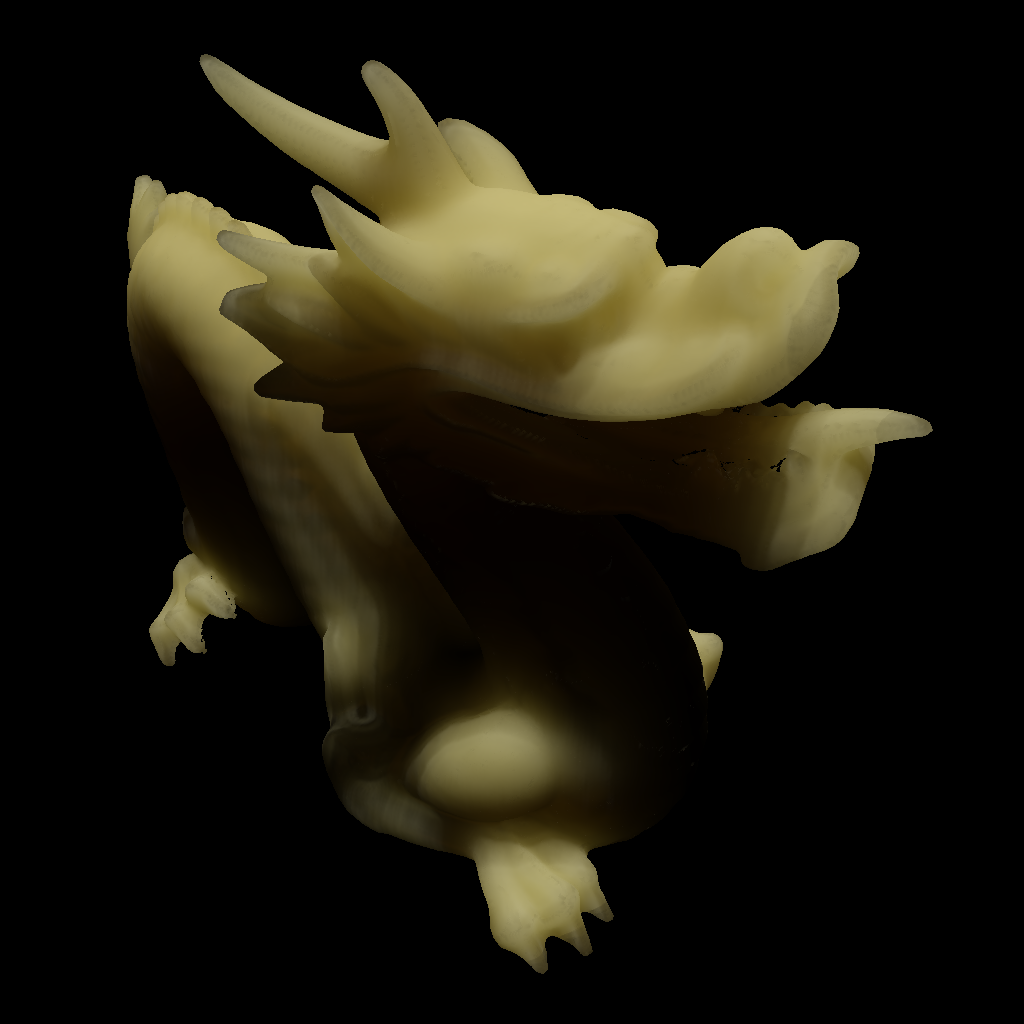
\includegraphics[width=0.4 \linewidth]{images/results/directional.png}
  \label{fig:dir_light_ex}
}
\subfloat[Point:  $\x_l = (0,0,2)$  $I_d = (18,18,18)$]{
  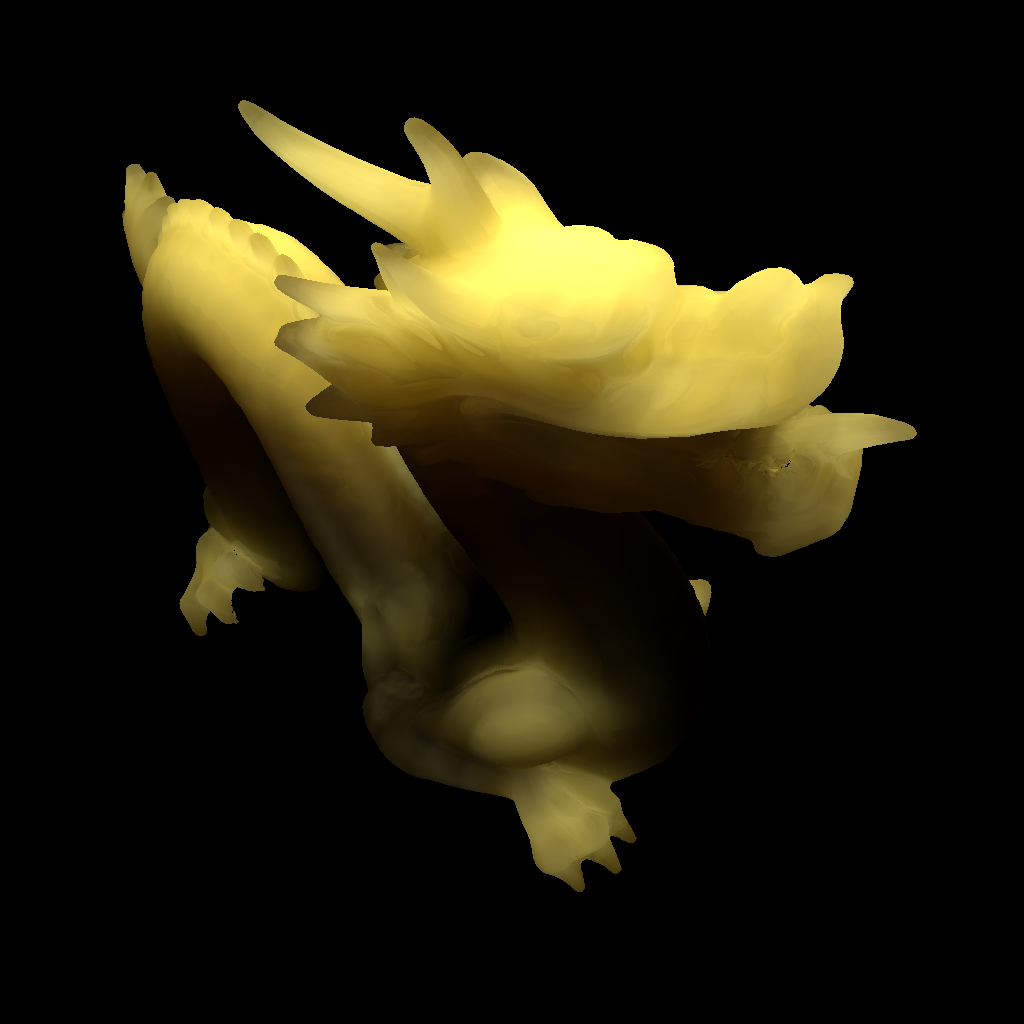
\includegraphics[width=0.4 \linewidth]{images/results/point.png}
  \label{fig:point_light_ex}
} 
\caption{Rendering with a directional and a point light. The material parameters are the ones for potato.}
\label{fig:dir_point_comparison}
\end{figure}
\FloatBarrier
\subsection{Rendering with environment light illumination}
\label{sec:envenv}
As for the environment lighting, we proceed as we outlined in Section \ref{sec:env}. In the method chapter, we omitted how we do actually organize and sample our CDF. The idea is to have one CDF for the rows of the function that gives us the CDF according to the probability $p_u(u)$. Then we have a CDF for each one of the column of the functions, that sample the probability $p_v(v|u)$. When we select a random couple of random points $(\zeta_1,\zeta_2)$ we first sample the first function according to $\zeta_1$, then we sample the resulting column using $\zeta_2$.

We define our discrete CDF as and array $C$ of $s+1$ elements as follows, where $s$ is the size of the distribution $P$ (that would be either $n$ or $m$ in our case). $P$ is an array of $N$ elements.
$$
C[i] = \frac{\sum_{k = 0}^{i-1} C[k]}{s\ C[s]}
$$
Then, we sample our CDF using a generic value $\zeta$ using the following:
$$
u = j + \frac{\zeta - C[j]}{C[j + 1] - C[j]}
$$
Where $j = \min_j\{j\ \in\ [0,s]\ |\ C[j] > \zeta \} - 1$ is the CDF value right before the CDF surpasses $\zeta$. This is basically the inverse function we discussed in Section \ref{sec:env}. Once we have calculated the two values $(u_1,u_2)$, as before we convert them to spherical coordinates, from which we create a set of directional lights that approximate our environment light. We can appreciate the rendering with different numbers of generated lights using the doge light map in Figure \ref{fig:doge_render_grape}.

\begin{figure}
\centering

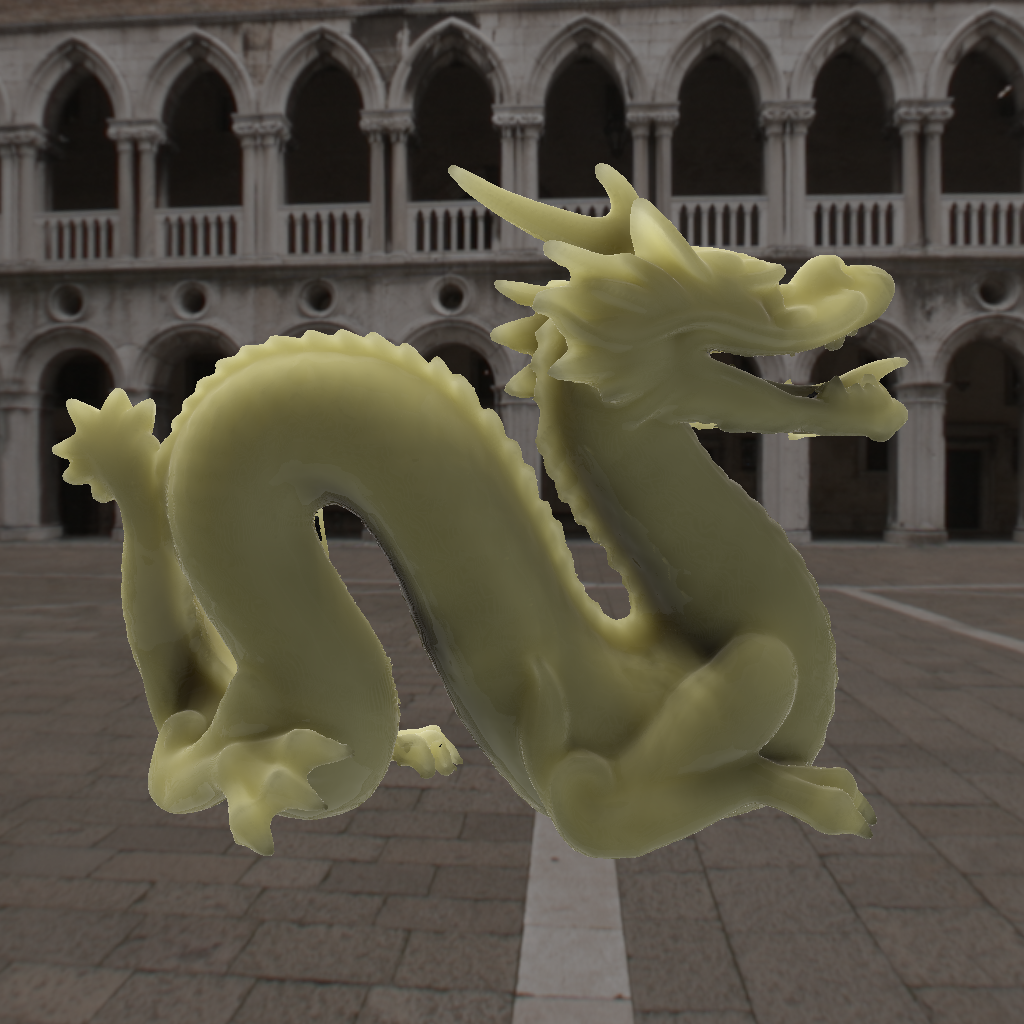
\includegraphics[width=0.9 \linewidth]{images/results/skymap_1.png}
\caption{Rendering a dragon using sixteen directional lights generated from the Doge map. The material parameters are for white grapefruit juice.}
\label{fig:doge_render_grape}
\end{figure}

\section{Discussion}
In this section, we anticipate some of the results that will be presented in Chapter \ref{chap:results}, in order to analyze our method and present advantages and disadvantages of the method, and more specifically of our implementation.

\subsection{Advantages}

The great advantage of this method, that comes from the BSSRDF model, is that it already accounts for self shadowing and self occlusion. So, no extra steps are required in order to account for these effects, that usually are difficult to evaluate in a real-time fashion. Moreover, if we reuse the same light map for all the objects in the scene, it is possible to account for the occlusion between objects. So, if an object is placed between the light and another object, a soft shadow of the first object on the second one will appear. However, since the material properties are not stored in the light map, the contribution from the other points will use the same properties that we are using to render the object (so, another object will cast a "potato shadow" on a potato object).  

Another advantage of our method is that is tightly coupled with the shadow mapping pipeline. Shadow mapping is widely used nowadays in most of real time graphics applications, so the cost of introducing our method is greatly reduced, since the light map data are usually available for use. In addition, the method is generally adaptable to any kind of shadow mapping technique, providing that it is able to store vertices and normals, and that those are accessible from step two in the algorithm. The cost of adding normal and vertex storage is usually only heavy on the memory requirements, since the vertex position is calculated anyway during the render to the shadow map. 

Compared to other techniques for rendering translucent materials (such as voxelization), our method has low memory requirements. As we will see, the size of the textures employed in the method should not be too big in order to achieve a reasonable quality. This also comes from the fact that subsurface scattering effects are result of blurring of the incoming light, so a low size texture can represent the effects very well.

Finally, another advantage of the method is that the final step relies only on the knowledge of the exiting position and normal, so it can be integrated in both a forward and a deferred rendering pipeline, making it very flexible.

\subsection{Disadvantages}
The first and biggest disadvantage of this method is that one frame is giving only an approximate and noisy approximation of the final result, that needs to be blurred using mipmaps in order to get a smooth result. In addition, every time something changed in the scene, the computations need to be redone every frame, not allowing the method to ever reach convergence. In this case, ping pong is not used at all, which results in a waste of precious memory space. The ping pong can be reused to account partially for the computation of the previous frame. In this way, the noise is reduced, at the price that the method is slower to react to swift changes of condition in the scene, generating ghosting artifacts.

As we can see in Figure TODO, it is difficult for our method to cover the whole surface of the object. The most hidden areas, such as the internal part of the dragon mouth, are not covered by any camera, and so the result are black holes on the surface. The problem is well known when acquiring an object from a 3D camera, where a rotation is often necessary in order to capture all the features of a mesh. A solution for this problem is to let the artist place the cameras himself/herself, but with an additional time effort. 

Another problem is that our method, relying on shadow mapping at its core, inherits all the defects and problems of shadow mapping. One of these is that constant shadow bias and offsets are sometimes not enough to cover the defects that inevitably generate when using this method. In addition, the artist must tweak this parameters in order to get a good result.  

Finally, a defect that comes from the method we are using to generate the directional lights from the environment map generally has the problem that in certain radiance maps, where there are a lot of very bright spots. In these maps, it tends to account only for the very bright spots and thus not approximate the overall result very well. In this case, a solution based on spherical harmonics \citep{peterpikeconference} environment lighting may be preferable.
